\addtocontents{toc}{\protect\setlength{\cftsecnumwidth}{13mm}}

\section{Casos de Uso}
A continuación, se describe cada caso de uso del PFG siguiendo el orden establecido en el cuadro \ref{tab:tabmapeo}.
\section{Gestionar Lugar}


\begin{longtable}{@{} p{3cm} p{10cm} @{}} \toprule
    \textbf{Caso de Uso}    & Gestionar Lugar \\ \midrule
    Actor                   & Gerente \\ \cmidrule{1-2}
    Descripción             & El gerente gestiona un Lugar. \\ \cmidrule{1-2}
    Propósito               & El gerente quiere registrar los datos de un nuevo Lugar. \\ \cmidrule{1-2}
    Precondiciones          & El gerente inicia su navegador web. \\ \cmidrule{1-2} 
    Postcondiciones         & Existe un nuevo Lugar. \\ \cmidrule{1-2} 
                            & 1. El gerente visita la página de Lugares. \\ 
                            & 2. El gerente hace click en el botón Nuevo. \\
   Curso Básico             & 3. El gerente ingresa la información correspondiente y envía los datos haciendo click en el botón Guardar. \\
                            & 4. El sistema registra el Lugar. \\ 
                            & 5. El sistema muestra la página de Lugares. \\ \cmidrule{1-2}
    Excepciones             & 1. El sistema no puede registrar el Lugar dada una falla en la base de datos. \\
                            & 2. El gerente puede salir de la página del formulario de Lugar en cualquier momento antes de Guardar haciendo click en Cancelar. \\ \bottomrule
   \caption{Caso de Uso - Gestionar Lugar (1)} \label{tab:tabcu-lug1} \\
   \end{longtable}


\begin{longtable}{@{} p{3cm} p{10cm} @{}} \toprule
    \textbf{Caso de Uso}    & Gestionar Lugar \\ \midrule
    Actor                   & Gerente \\ \cmidrule{1-2}
    Descripción             & El gerente gestiona un Lugar. \\ \cmidrule{1-2}
    Propósito               & El gerente quiere modificar los datos de un Lugar. \\ \cmidrule{1-2}
    Precondiciones          & El gerente inicia su navegador web. \\
                            & Existe el Lugar. \\ \cmidrule{1-2} 
    Postcondiciones         & Existe un Lugar con nuevos datos. \\ \cmidrule{1-2} 
                            & 1. El gerente visita la página de Lugar. \\ 
                            & 2. El gerente hace click en el botón Modificar de un Lugar. \\
   Curso Básico             & 2.1 El sistema recuperara datos de la Lugar para intentar poblar el formulario de Lugar. \\
                            & 3. El gerente ingresa la información correspondiente y envía los datos haciendo click en el botón Guardar. \\
                            & 4. El sistema actualiza el Lugar. \\ 
                            & 5. El sistema muestra la página de Lugares. \\ \cmidrule{1-2}
    Excepciones             & 1. El sistema no puede actualizar el Lugar dada una falla en la base de datos. \\
                            & 2. El gerente puede salir de la página del formulario de Lugar en cualquier momento antes de Guardar haciendo click en Cancelar. \\ \bottomrule
   \caption{Caso de Uso - Gestionar Lugar (2)} \label{tab:tabcu-lug2} \\
   \end{longtable}



\begin{longtable}{@{} p{3cm} p{10cm} @{}} \toprule
    \textbf{Caso de Uso}    & Gestionar Lugar \\ \midrule
    Actor                   & Gerente \\ \cmidrule{1-2}
    Descripción             & El gerente gestiona un Lugar. \\ \cmidrule{1-2}
    Propósito               & El gerente quiere eliminar un Lugar. \\ \cmidrule{1-2}
    Precondiciones          & El gerente inicia su navegador web. \\
                            & Existe el Lugar. \\ \cmidrule{1-2} 
    Postcondiciones         & Se eliminó un Lugar. \\ \cmidrule{1-2} 
                            & 1. El gerente visita la página de Lugares. \\ 
                            & 2. El gerente hace click en el botón Detalles de un Lugar. \\
                            & 2.1 El sistema recupera los datos del Lugar para mostrar la página de detalles. \\
    Curso Básico            & 3. El gerente hace click en el botón Eliminar. \\
                            & 4. El sistema elimina el Lugar. \\ 
                            & 5. El sistema muestra la página de Lugares. \\ \cmidrule{1-2}
    Excepciones             & 1. El sistema no puede eliminar el Lugar dada una falla en la base de datos. \\
                            & 2. El gerente puede salir de la página del formulario de Lugar en cualquier momento antes de eliminar haciendo click en Cancelar. \\ \bottomrule
   \caption{Caso de Uso - Gestionar Lugar (3)} \label{tab:tabcu-lug3} \\
   \end{longtable}

    \begin{figure}[H]
        \centering
        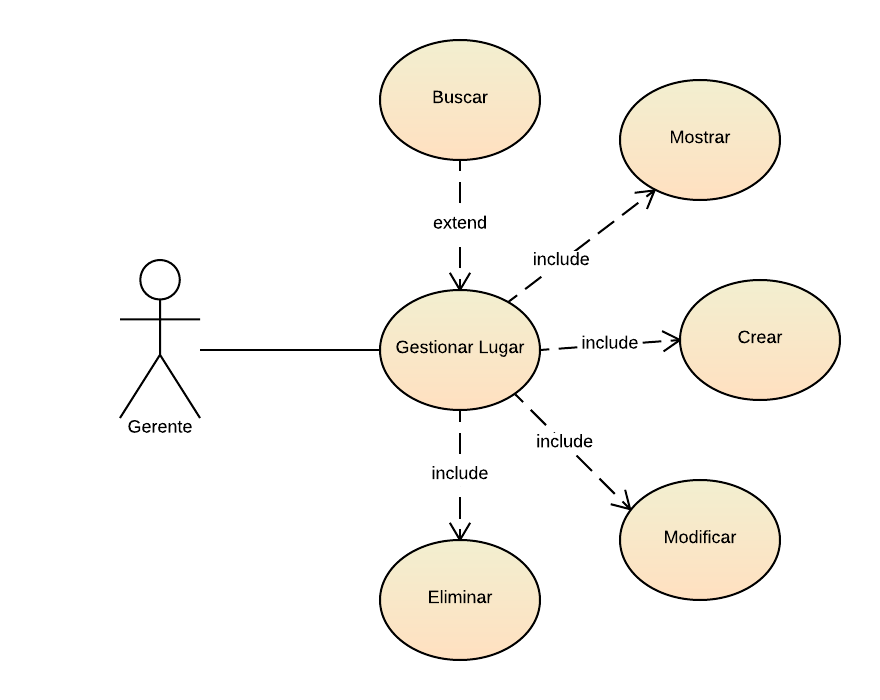
\includegraphics[width=0.85\textwidth]{chapter10/lugar-uc}
        \caption{Diagrama de Caso de Uso - Gestionar Lugar}
        \label{fig:lugar-uc}
    \end{figure}
    
    \begin{figure}[H]
        \centering
        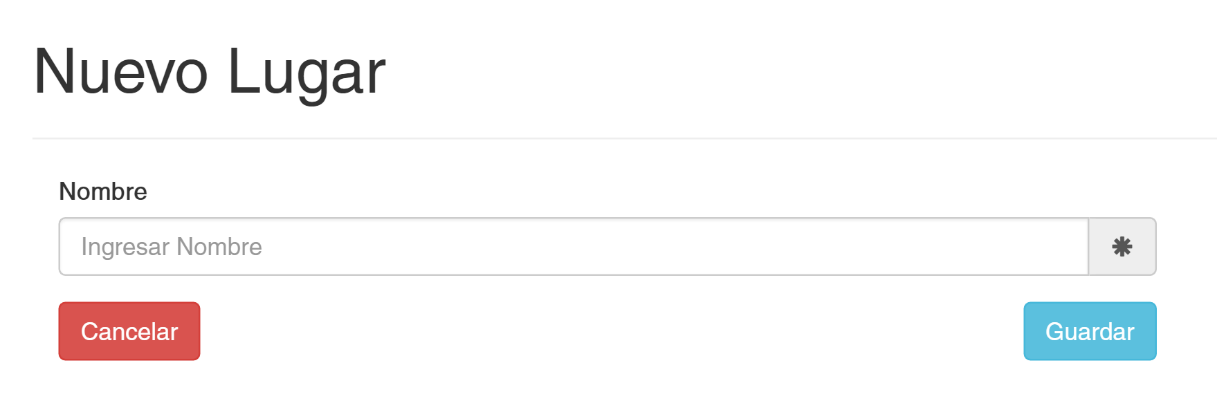
\includegraphics[width=1\textwidth]{chapter10/lugar-int}
        \caption{Interfaz Tentativa - Gestionar Lugar}
        \label{fig:lugar-int}
    \end{figure}
    
 \begin{landscape}
        \begin{figure}[H]
        \centering
        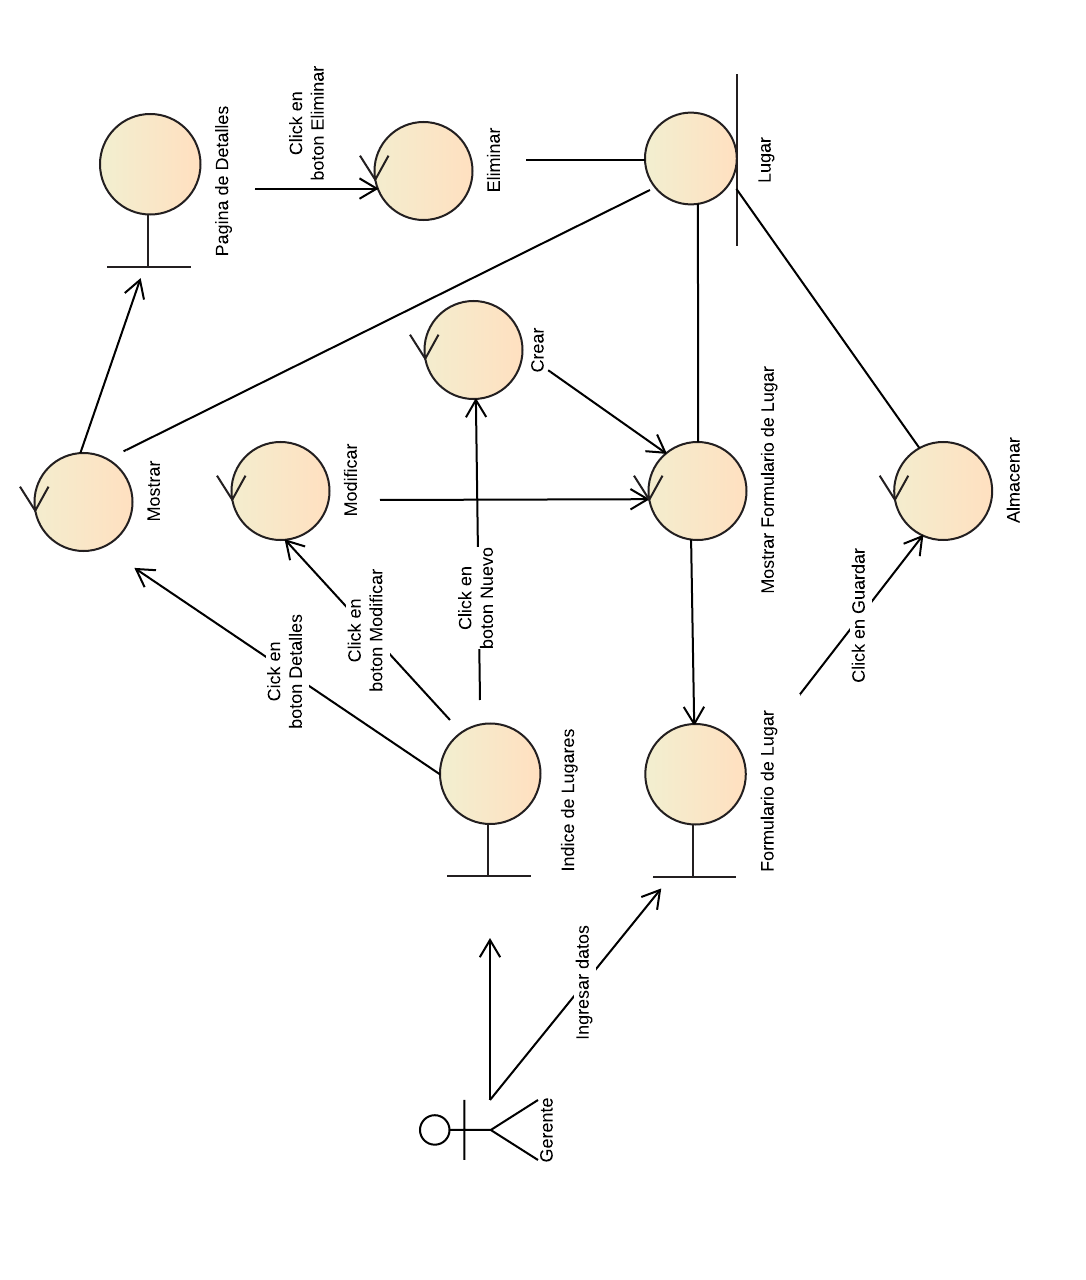
\includegraphics[width=1\textwidth]{chapter10/lugar-rob}
        \caption{Diagrama de Robustez - Gestionar Lugar}
        \label{fig:lugar-rob}
    \end{figure}
    
    \begin{figure}[H]
        \centering
        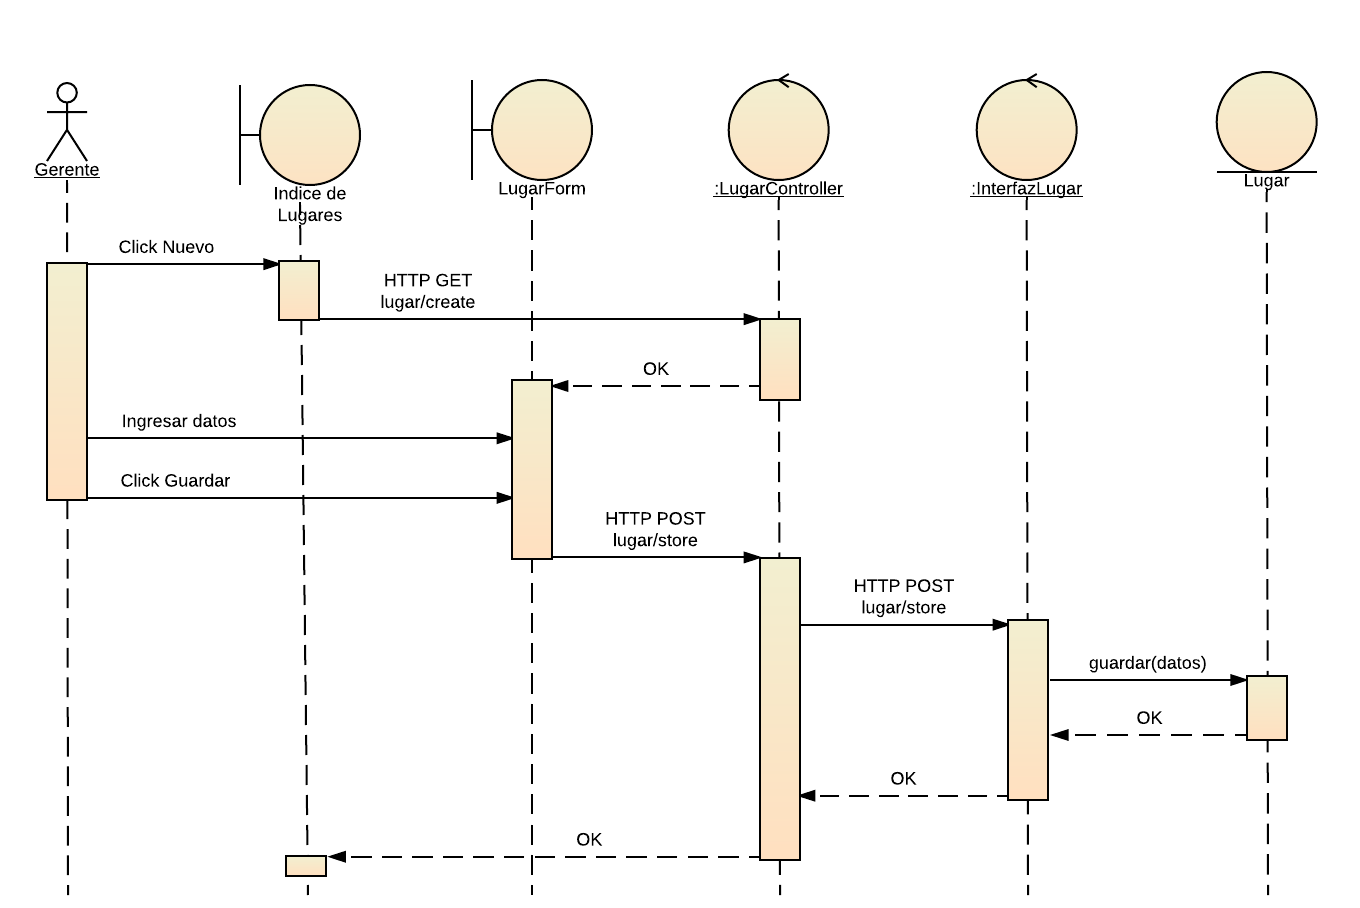
\includegraphics[width=1.2\textwidth]{chapter10/lugar-seq-create}
        \caption{Diagrama de Secuencia - Gestionar Lugar (1)}
        \label{fig:lugar-seq-create}
    \end{figure}
    
    \begin{figure}[H]
        \centering
        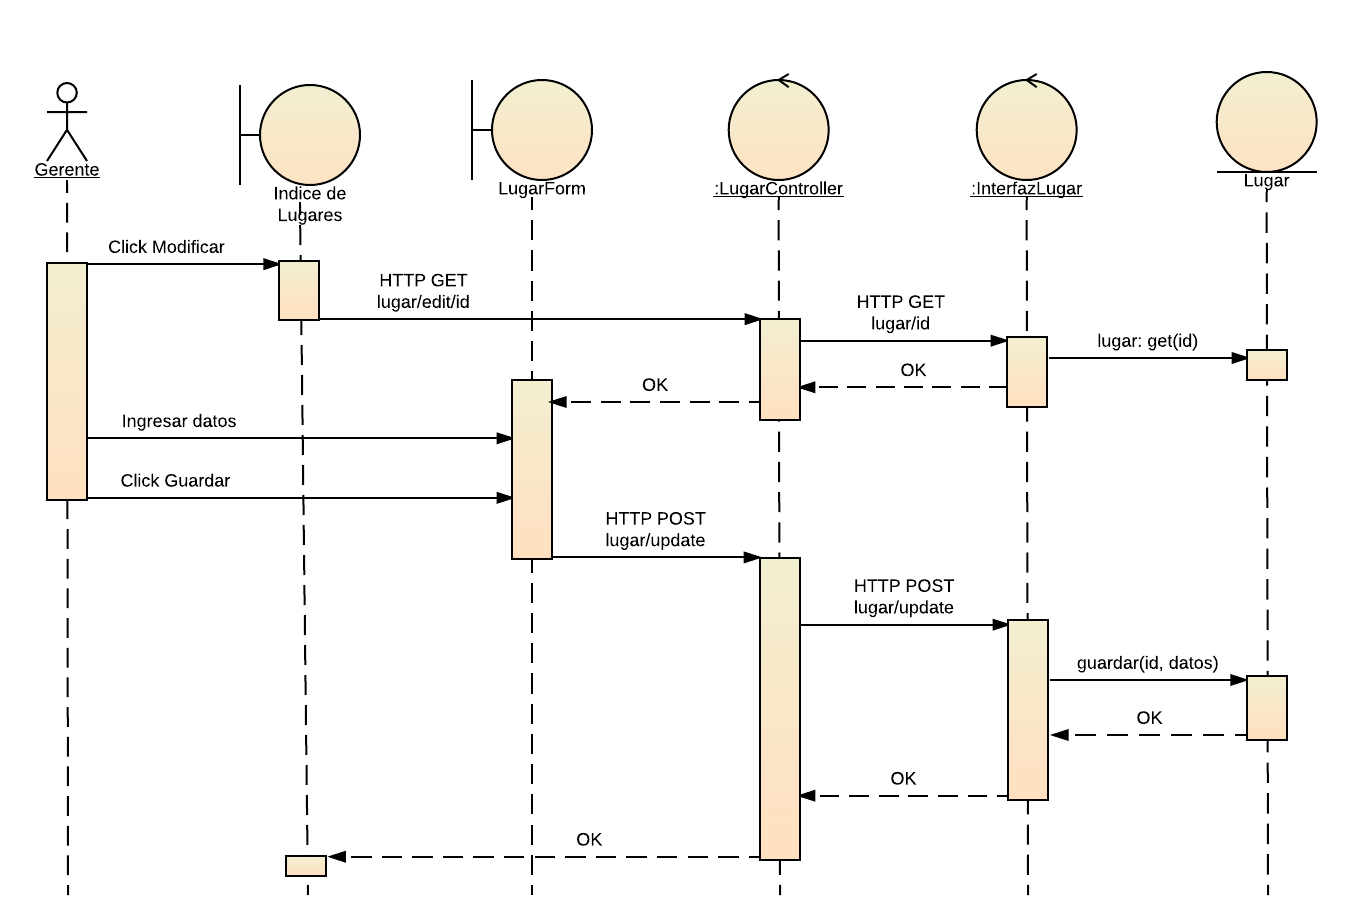
\includegraphics[width=1.2\textwidth]{chapter10/lugar-seq-edit}
        \caption{Diagrama de Secuencia - Gestionar Lugar (2)}
        \label{fig:lugar-seq-edit}
    \end{figure}
    
    \begin{figure}[H]
        \centering
        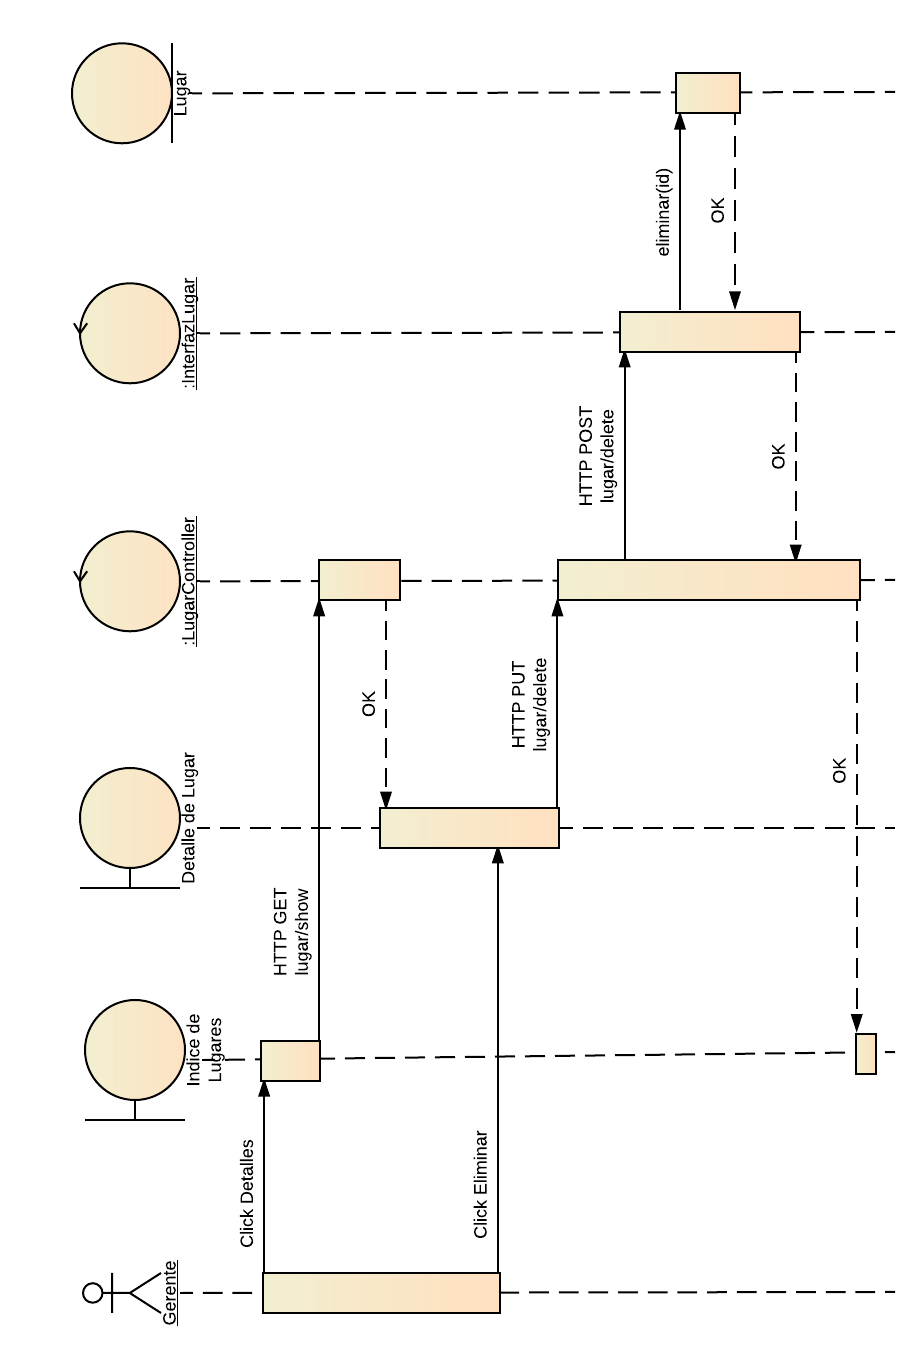
\includegraphics[width=1.2\textwidth]{chapter10/lugar-seq-del}
        \caption{Diagrama de Secuencia - Gestionar Lugar (3)}
        \label{fig:lugar-seq-del}
    \end{figure}
 \end{landscape}

\section{Gestionar Cámara}

\begin{longtable}{@{} p{3cm} p{10cm} @{}} \toprule
    \textbf{Caso de Uso}    & Gestionar Cámara \\ \midrule
    Actor                   & Gerente \\ \cmidrule{1-2}
    Descripción             & El gerente gestiona una Cámara. \\ \cmidrule{1-2}
    Propósito               & El gerente quiere registrar los datos de una nueva Cámara. \\ \cmidrule{1-2}
    Precondiciones          & El gerente inicia su navegador web. \\
                            & Existe el lugar. \\ \cmidrule{1-2} 
    Postcondiciones         & Existe una nueva Cámara. \\ \cmidrule{1-2} 
                            & 1. El gerente visita la página de Cámaras. \\ 
                            & 2. El gerente hace click en el botón Nuevo. \\
   Curso Básico             & 3. El gerente ingresa la información correspondiente y envía los datos haciendo click en el botón Guardar. \\
                            & 4. El sistema registra la Cámara. \\ 
                            & 5. El sistema muestra la página de Cámaras. \\ \cmidrule{1-2}
    Excepciones             & 1. El sistema no puede registrar la Cámara dada una falla en la base de datos. \\
                            & 2. El gerente puede salir de la página del formulario de Cámara en cualquier momento antes de Guardar haciendo click en Cancelar. \\ \bottomrule
   \caption{Caso de Uso - Gestionar Cámara (1)} \label{tab:tabcu-cam1} \\
   \end{longtable}


\begin{longtable}{@{} p{3cm} p{10cm} @{}} \toprule
    \textbf{Caso de Uso}    & Gestionar Cámara \\ \midrule
    Actor                   & Gerente \\ \cmidrule{1-2}
    Descripción             & El gerente gestiona una Cámara. \\ \cmidrule{1-2}
    Propósito               & El gerente quiere modificar los datos de una Cámara. \\ \cmidrule{1-2}
    Precondiciones          & El gerente inicia su navegador web. \\
                            & Existe el lugar. \\
                            & Existe la Cámara. \\ \cmidrule{1-2} 
    Postcondiciones         & Existe una Cámara con nuevos datos. \\ \cmidrule{1-2} 
                            & 1. El gerente visita la página de Cámaras. \\ 
                            & 2. El gerente hace click en el botón Modificar de una Cámara. \\
   Curso Básico             & 2.1 El sistema recuperara datos de la Cámara para intentar poblar el formulario de Cámara. \\
                            & 3. El gerente ingresa la información correspondiente y envía los datos haciendo click en el botón Guardar. \\
                            & 4. El sistema actualiza la Cámara. \\ 
                            & 5. El sistema muestra la página de Cámaras. \\ \cmidrule{1-2}
    Excepciones             & 1. El sistema no puede actualizar la Cámara dada una falla en la base de datos. \\
                            & 2. El gerente puede salir de la página del formulario de Cámara en cualquier momento antes de Guardar haciendo click en Cancelar. \\ \bottomrule
   \caption{Caso de Uso - Gestionar Cámara (2)} \label{tab:tabcu-cam2} \\
   \end{longtable}



\begin{longtable}{@{} p{3cm} p{10cm} @{}} \toprule
    \textbf{Caso de Uso}    & Gestionar Cámara \\ \midrule
    Actor                   & Gerente \\ \cmidrule{1-2}
    Descripción             & El gerente gestiona una Cámara. \\ \cmidrule{1-2}
    Propósito               & El gerente quiere eliminar una Cámara. \\ \cmidrule{1-2}
    Precondiciones          & El gerente inicia su navegador web. \\
                            & Existe el lugar. \\
                            & Existe la Cámara. \\ \cmidrule{1-2} 
    Postcondiciones         & Se eliminó una Cámara. \\ \cmidrule{1-2} 
                            & 1. El gerente visita la página de Cámaras. \\ 
                            & 2. El gerente hace click en el botón Detalles de un Cámara. \\
                            & 2.1 El sistema recupera los datos de la Cámara para mostrar la página de detalles. \\
    Curso Básico            & 3. El gerente hace click en el boton Eliminar. \\
                            & 4. El sistema muestra la página del Formulario de Cámara. \\
                            & 6. El sistema elimina la Cámara. \\ 
                            & 7. El sistema muestra la página de Cámaras. \\ \cmidrule{1-2}
    Excepciones             & 1. El sistema no puede eliminar la Cámara dada una falla en la base de datos. \\
                            & 2. El gerente puede salir de la página del formulario de Cámara en cualquier momento antes de eliminar haciendo click en Cancelar. \\ \bottomrule
   \caption{Caso de Uso - Gestionar Cámara (3)} \label{tab:tabcu-cam3} \\
   \end{longtable}

    
    
    \begin{figure}[H]
        \centering
        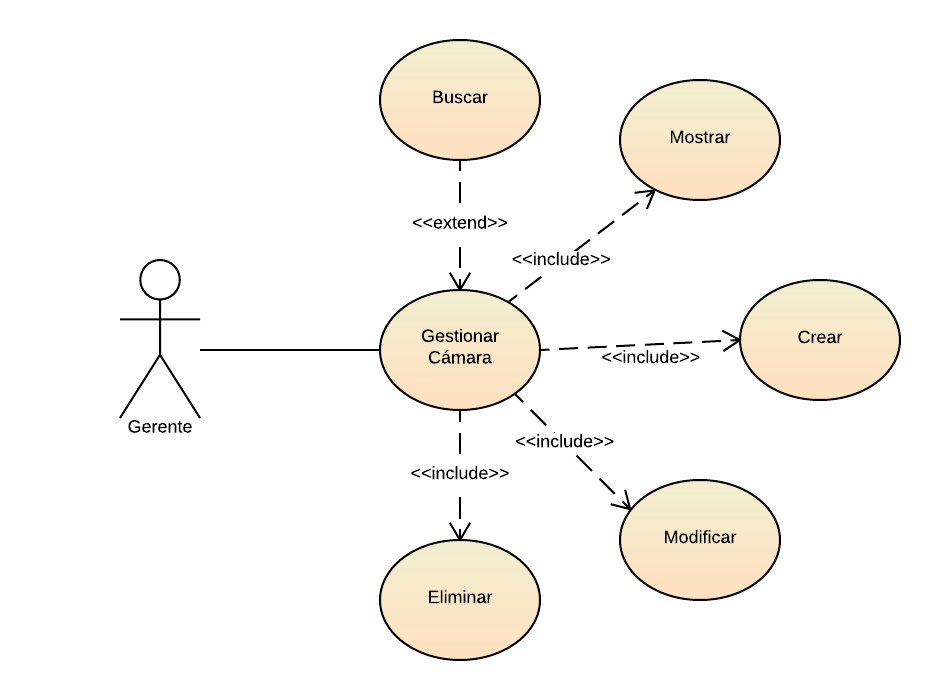
\includegraphics[width=0.85\textwidth]{chapter10/uc-cam}
        \caption{Diagrama de Caso de Uso - Gestionar Cámara}
        \label{fig:uc-cam}
    \end{figure}
    
      \begin{figure}[H]
        \centering
        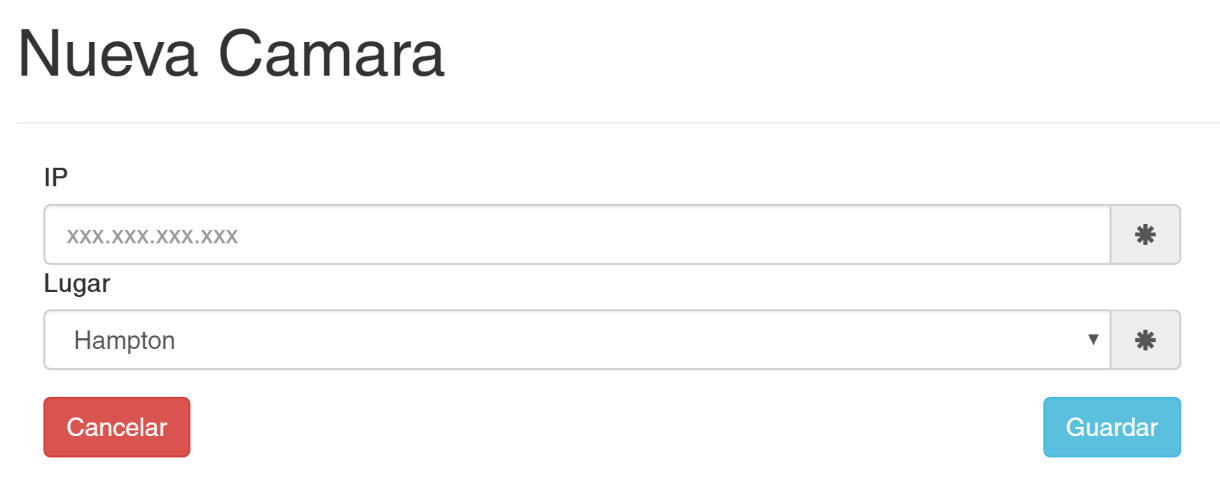
\includegraphics[width=0.85\textwidth]{chapter10/int-cam}
        \caption{Interfaz de Usuario Tentativa - Gestionar Cámara}
        \label{fig:int-cam}
    \end{figure}
    
\begin{landscape}
    \begin{figure}[H]
        \centering
        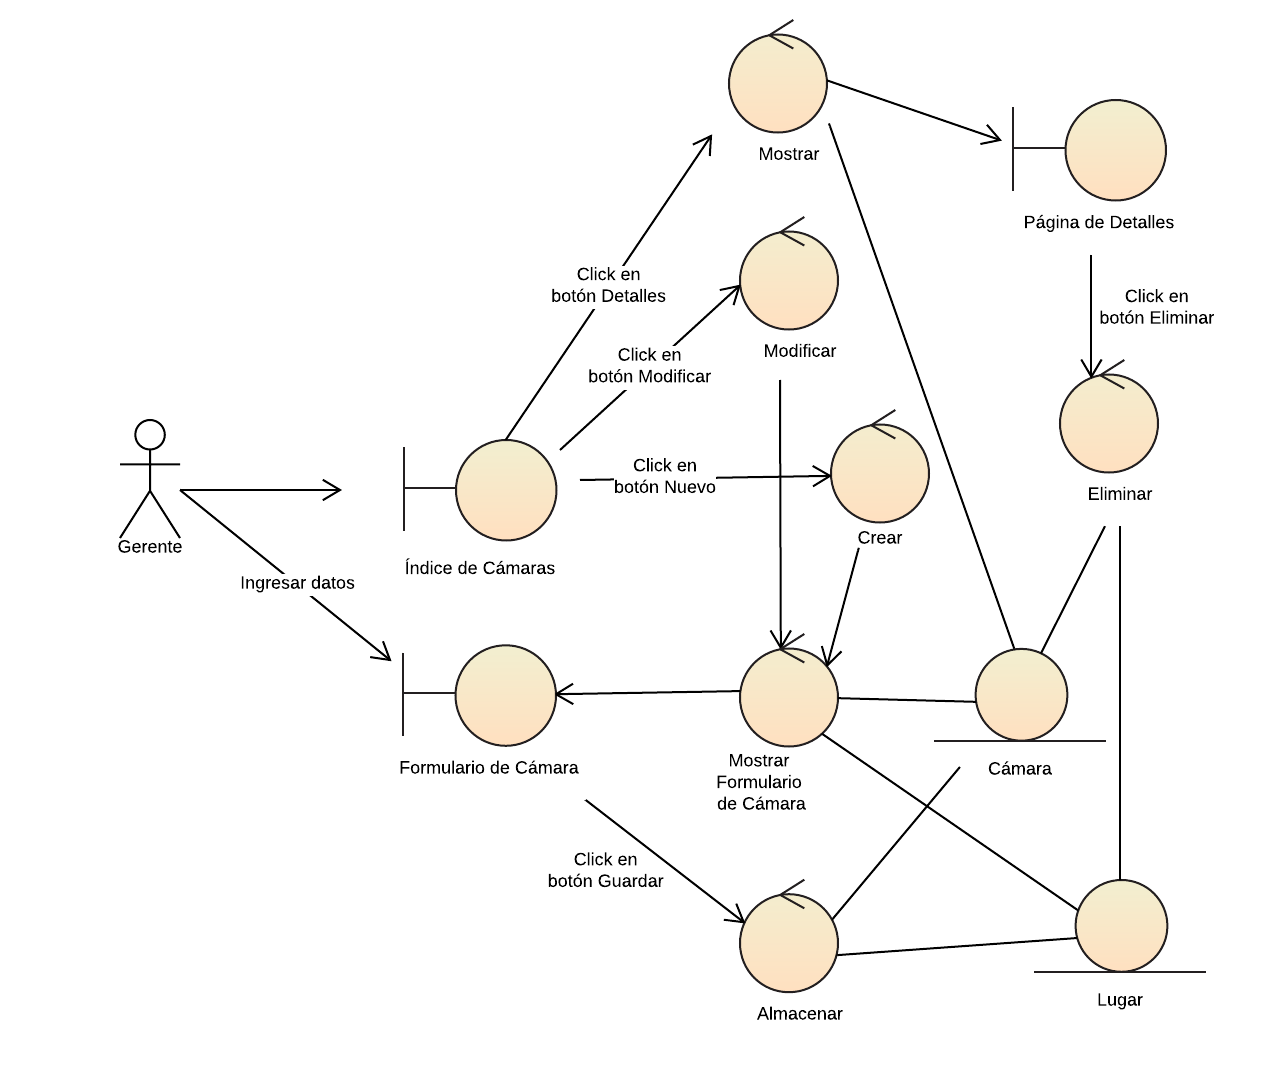
\includegraphics[width=1\textwidth]{chapter10/rob-cam}
        \caption{Diagrama de Robustez - Gestionar Cámara }
        \label{fig:rob-cam}
    \end{figure}
  
    \begin{figure}[H]
        \centering
        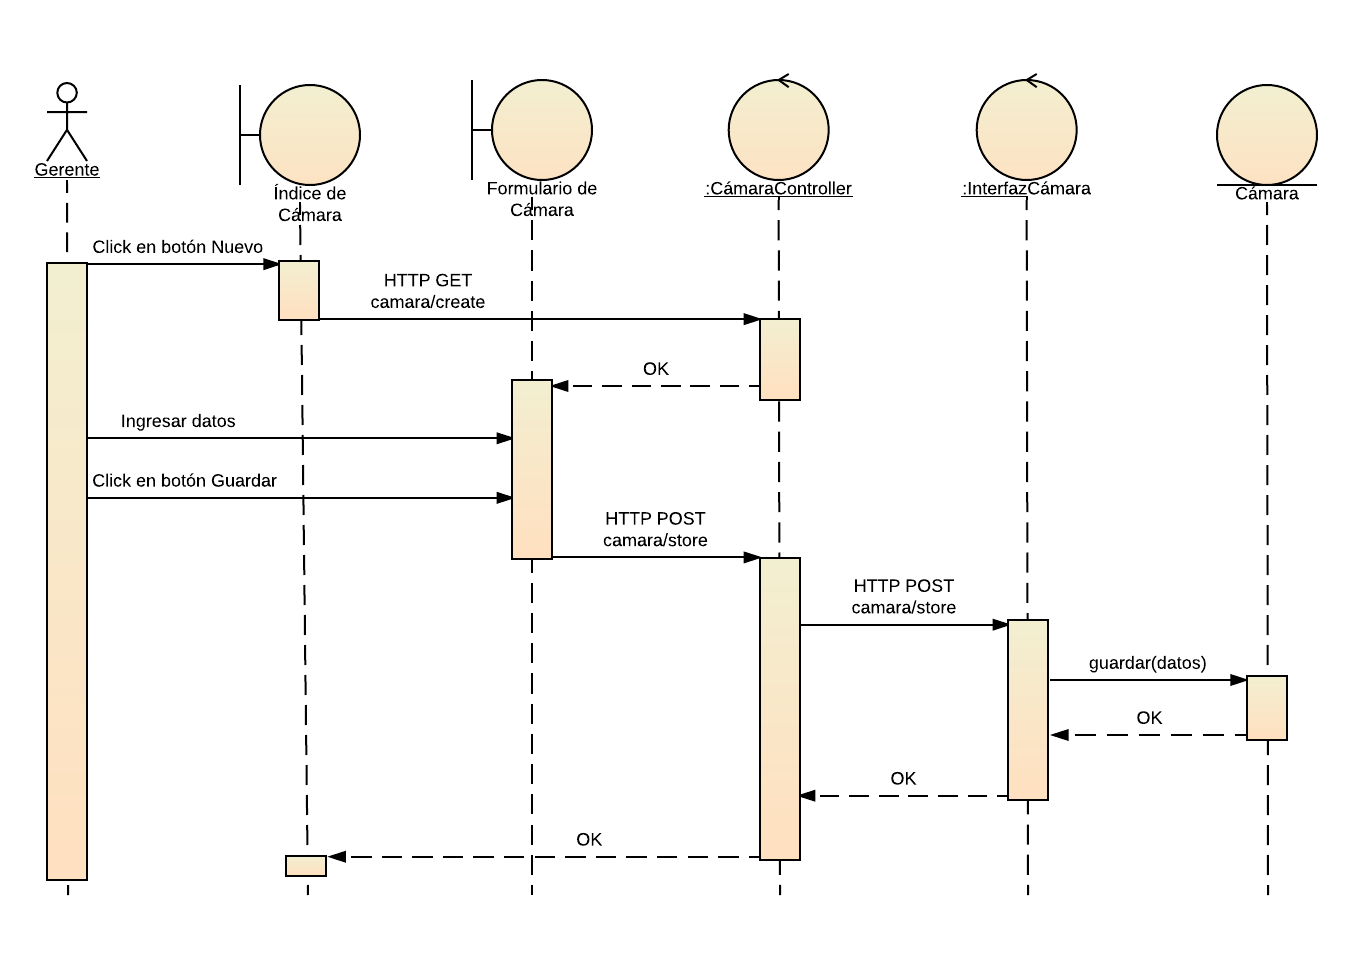
\includegraphics[width=1.2\textwidth]{chapter10/seq-cam-nu}
        \caption{Diagrama de Secuencia - Gestionar Cámara (1) }
        \label{fig:seq-cam-nu}
    \end{figure}
    
    \begin{figure}[H]
        \centering
        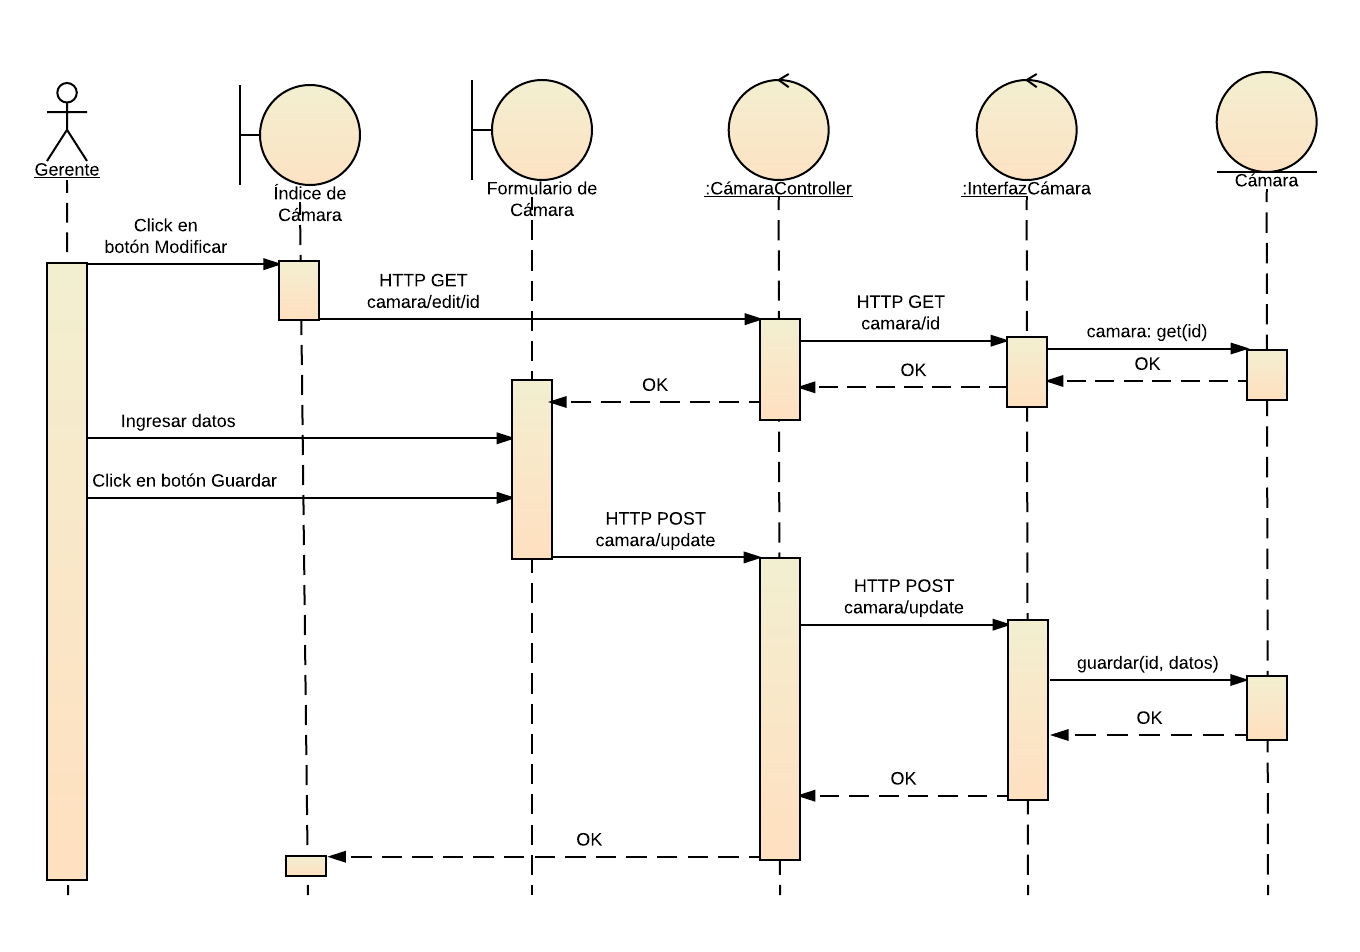
\includegraphics[width=1.21\textwidth]{chapter10/seq-cam-mo}
        \caption{Diagrama de Secuencia - Gestionar Cámara (2) }
        \label{fig:seq-cam-mo}
    \end{figure}
    
    \begin{figure}[H]
        \centering
        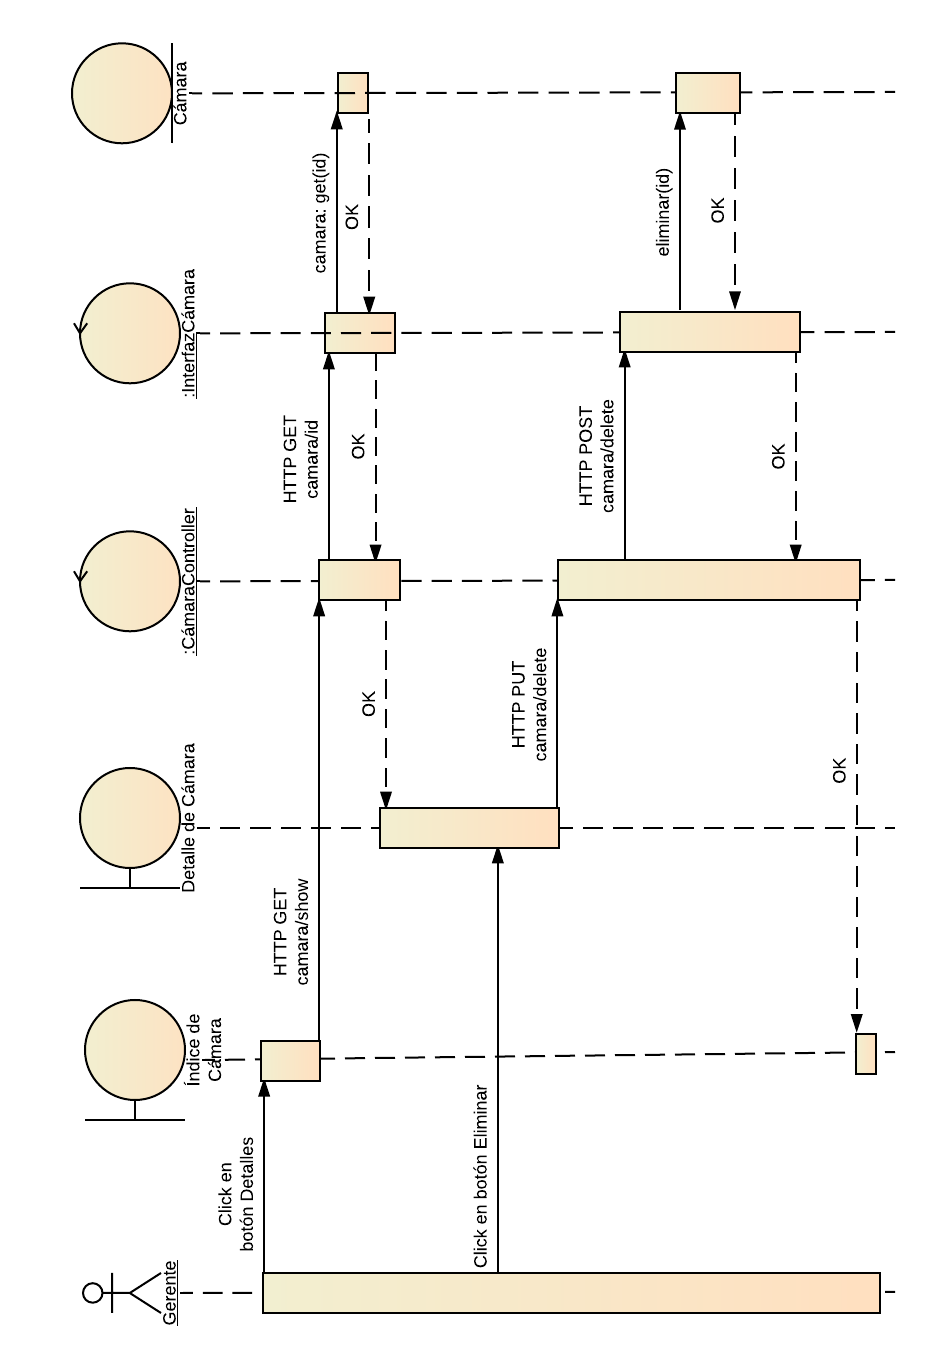
\includegraphics[width=1.2\textwidth]{chapter10/seq-cam-el}
        \caption{Diagrama de Secuencia - Gestionar Cámara (3) }
        \label{fig:seq-cam-el}
    \end{figure}
    \end{landscape}

\section{Gestionar Matrícula}

\begin{longtable}{@{} p{3cm} p{10cm} @{}} \toprule
    \textbf{Caso de Uso}    & Gestionar Matrícula \\ \midrule
    Actor                   & Gerente \\ \cmidrule{1-2}
    Descripción             & El gerente gestiona una Matrícula. \\ \cmidrule{1-2}
    Propósito               & El gerente quiere gestionar una Matrícula. \\ \cmidrule{1-2}
    Precondiciones          & El gerente inicia su navegador web. Existe el Propietario. Existe la Matrícula. \\ \cmidrule{1-2} 
    Postcondiciones         & Existe una nueva Matrícula. \\ \cmidrule{1-2} 
                            & 1. El gerente visita la página de Propietarios. \\ 
                            & 2. El gerente hace click en el botón Detalles de un Propietario. \\
                            & 2.1 El sistema recupera los datos del Propietario para mostrar la página de detalles. \\
    Curso Básico            & 3. El gerente hace click en el boton Nuevo. \\
                            & 4. El sistema muestra la página del Formulario de Matrícula. \\
                            & 5. El gerente ingresa la información correspondiente y envía los datos haciendo click en el botón Guardar. \\ 
                            & 6. El sistema registra la Matrícula. \\ 
                            & 7. El sistema muestra la página de Detalles del Propietario con la nueva Matrícula. \\ \cmidrule{1-2}
    Excepciones             & 1. El sistema no puede registrar la Matrícula dada una falla en la base de datos. \\
                            & 2. El gerente puede salir de la página del formulario de Matrícula en cualquier momento antes de eliminar haciendo click en Cancelar. \\ \bottomrule
   \caption{Caso de Uso - Gestionar Matrícula (1} \label{tab:tabcu-matri1} \\
   \end{longtable}

\begin{longtable}{@{} p{3cm} p{10cm} @{}} \toprule
    \textbf{Caso de Uso}    & Gestionar Matrícula \\ \midrule
    Actor                   & Gerente \\ \cmidrule{1-2}
    Descripción             & El gerente gestiona una Matrícula. \\ \cmidrule{1-2}
    Propósito               & El gerente quiere gestionar una Matrícula. \\ \cmidrule{1-2}
    Precondiciones          & El gerente inicia su navegador web. Existe el Propietario. Existe la Matrícula. \\ \cmidrule{1-2} 
    Postcondiciones         & Existe una Matrícula con nuevos datos. \\ \cmidrule{1-2} 
                            & 1. El gerente visita la página de Propietarios. \\ 
                            & 2. El gerente hace click en el botón Detalles de un Propietario. \\
                            & 2.1 El sistema recupera los datos del Propietario para mostrar la página de detalles. \\
    Curso Básico            & 3. El gerente hace click en el boton Modificar de una Matrícula. \\
                            & 4. El sistema muestra la página del Formulario de Matrícula. \\
                            & 4.1. El sistema recupera datos de la Matrícula para intentar poblar el formulario. \\
                            & 6. El gerente ingresa la información correspondiente y envía los datos haciendo click en el botón Guardar. \\ 
                            & 7. El sistema actualiza la Matrícula. \\ 
                            & 8. El sistema muestra la página de Detalles del Propietario con la nueva Matrícula. \\ \cmidrule{1-2}
    Excepciones             & 1. El sistema no puede actualizar la Matrícula dada una falla en la base de datos. \\
                            & 2. El gerente puede salir de la página del formulario de Matrícula en cualquier momento antes de eliminar haciendo click en Cancelar. \\ \bottomrule
   \caption{Caso de Uso - Gestionar Matrícula (2)} \label{tab:tabcu-matri2} \\
   \end{longtable}

 \begin{longtable}{@{} p{3cm} p{10cm} @{}} \toprule
    \textbf{Caso de Uso}    & Gestionar Matrícula \\ \midrule
    Actor                   & Gerente \\ \cmidrule{1-2}
    Descripción             & El gerente gestiona una Matrícula. \\ \cmidrule{1-2}
    Propósito               & El gerente quiere gestionar una Matrícula. \\ \cmidrule{1-2}
    Precondiciones          & El gerente inicia su navegador web. Existe el Propietario. Existe la Matrícula. \\ \cmidrule{1-2} 
    Postcondiciones         & Se eliminó una Matrícula. \\ \cmidrule{1-2} 
                            & 1. El gerente visita la página de Propietarios. \\ 
                            & 2. El gerente hace click en el botón Detalles de un Propietario. \\
                            & 2.1 El sistema recupera los datos del Propietario para mostrar la página de detalles. \\
    Curso Básico            & 3. El gerente selecciona una Matrícula haciendo click en ell boton Detalles. \\
                            & 4. El sistema muestra la página de Detalles de una Matrícula. \\
                            & 5. El gerente elimina la Matrícula haciendo click en el botón Eliminar. \\
                            & 6. El sistema elimina la Matrícula. \\ \cmidrule{1-2}
    Excepciones             & 1. El sistema no puede eliminar la Matrícula dada una falla en la base de datos. \\
                            & 2. El gerente puede salir de la página de detalles en cualquier momento antes de eliminar haciendo click en Cancelar. \\ \bottomrule
   \caption{Caso de Uso - Gestionar Matrícula (3)} \label{tab:tabcu-matri3} \\
   \end{longtable}
  
 
    \begin{figure}[H]
        \centering
        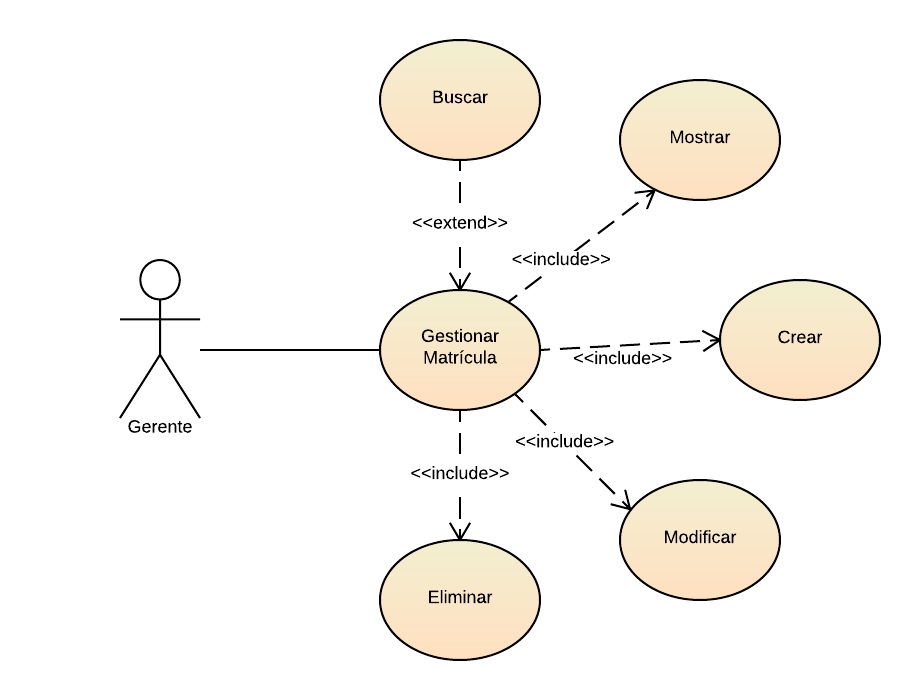
\includegraphics[width=0.8\textwidth]{chapter10/uc-matri}
        \caption{Diagrama de Caso de Uso - Gestionar Matrícula}
        \label{fig:uc-matri}
    \end{figure}
    
     \begin{figure}[H]
        \centering
        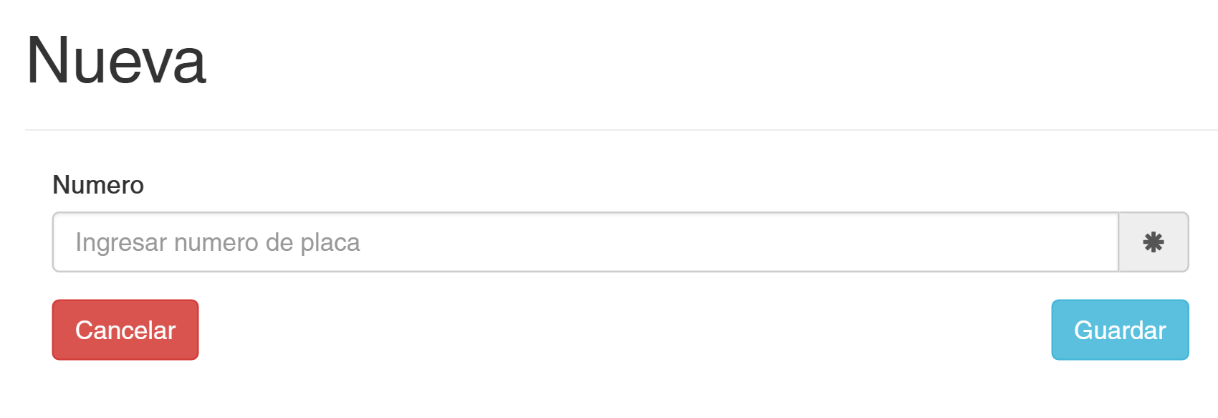
\includegraphics[width=0.85\textwidth]{chapter10/int-matri}
        \caption{Interfaz de Usuario Tentativa - Gestionar Matrícula}
        \label{fig:int-matri}
    \end{figure}
    
\begin{landscape}
    \begin{figure}[H]
        \centering
        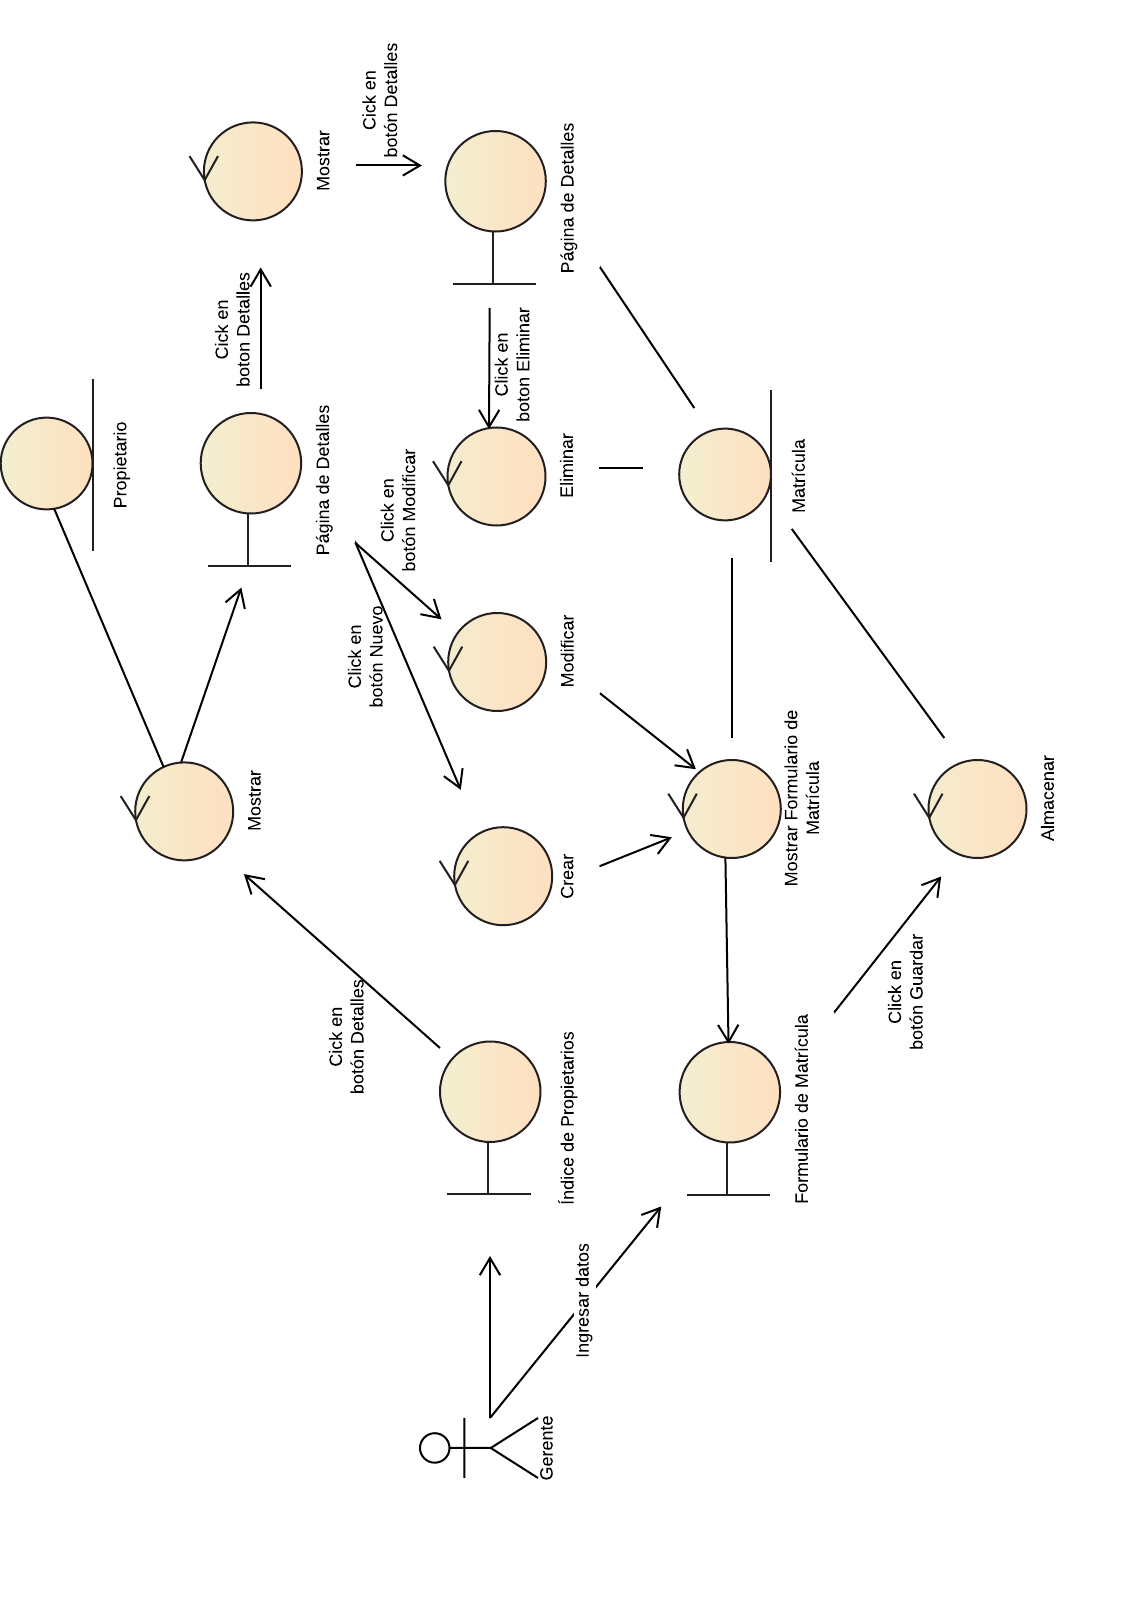
\includegraphics[width=1.1\textwidth]{chapter10/rob-matri}
        \caption{Diagrama de Robustez - Gestionar Matrícula}
        \label{fig:rob-matri}
    \end{figure}
    \begin{figure}[H]
        \centering
        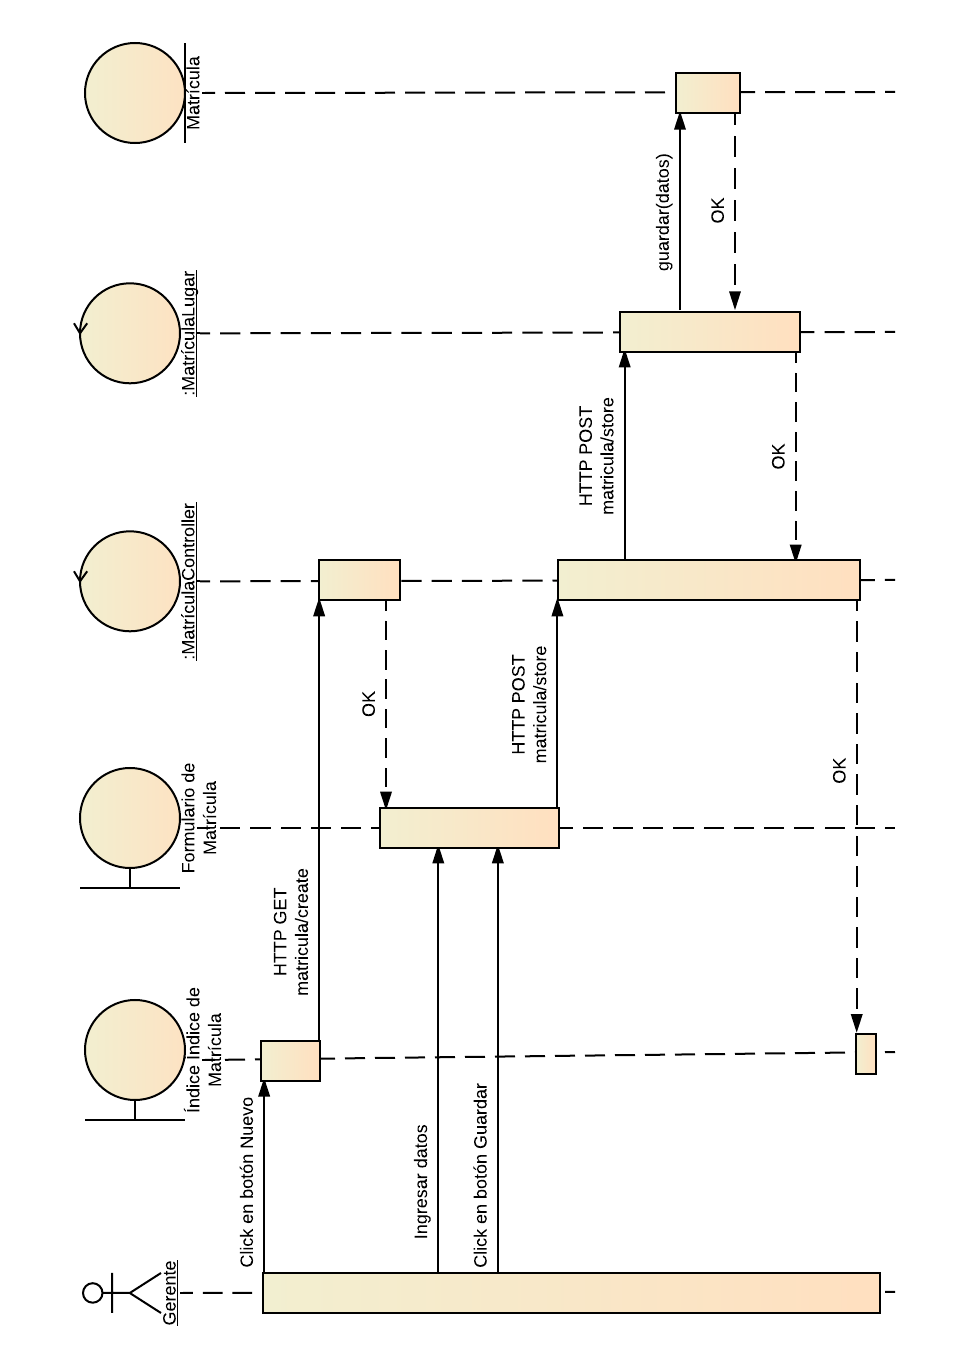
\includegraphics[width=1.2\textwidth]{chapter10/seq-matri-nu}
        \caption{Diagrama de Secuencia - Gestionar Matrícula (1) }
        \label{fig:seq-matri-nu}
    \end{figure}
    
    \begin{figure}[H]
        \centering
        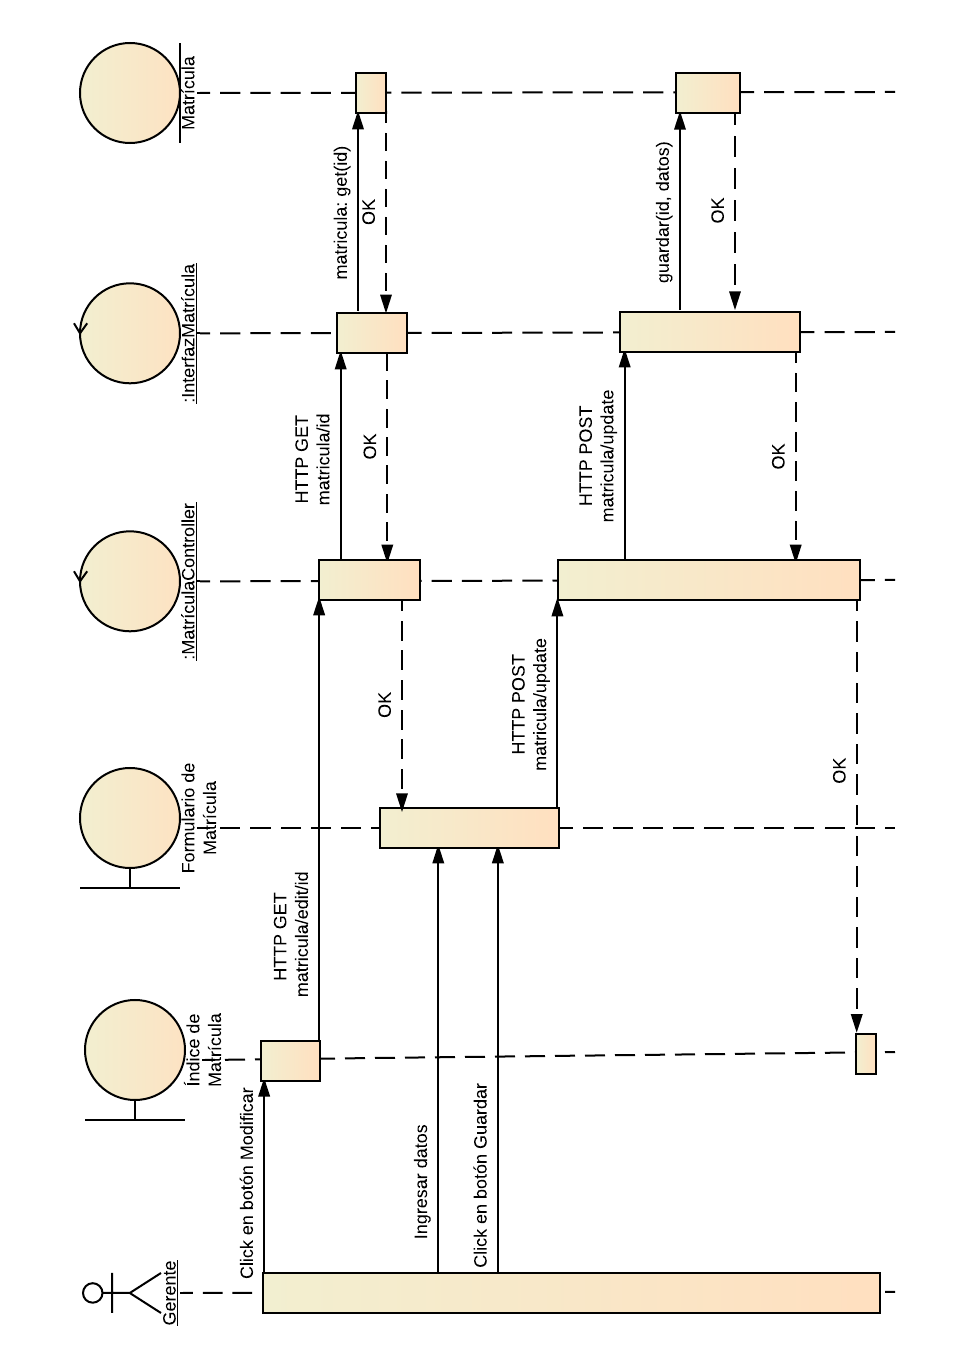
\includegraphics[width=1.2\textwidth]{chapter10/seq-matri-mod}
        \caption{Diagrama de Secuencia - Gestionar Matrícula (2) }
        \label{fig:seq-matri-mo}
    \end{figure}
    
    \begin{figure}[H]
        \centering
        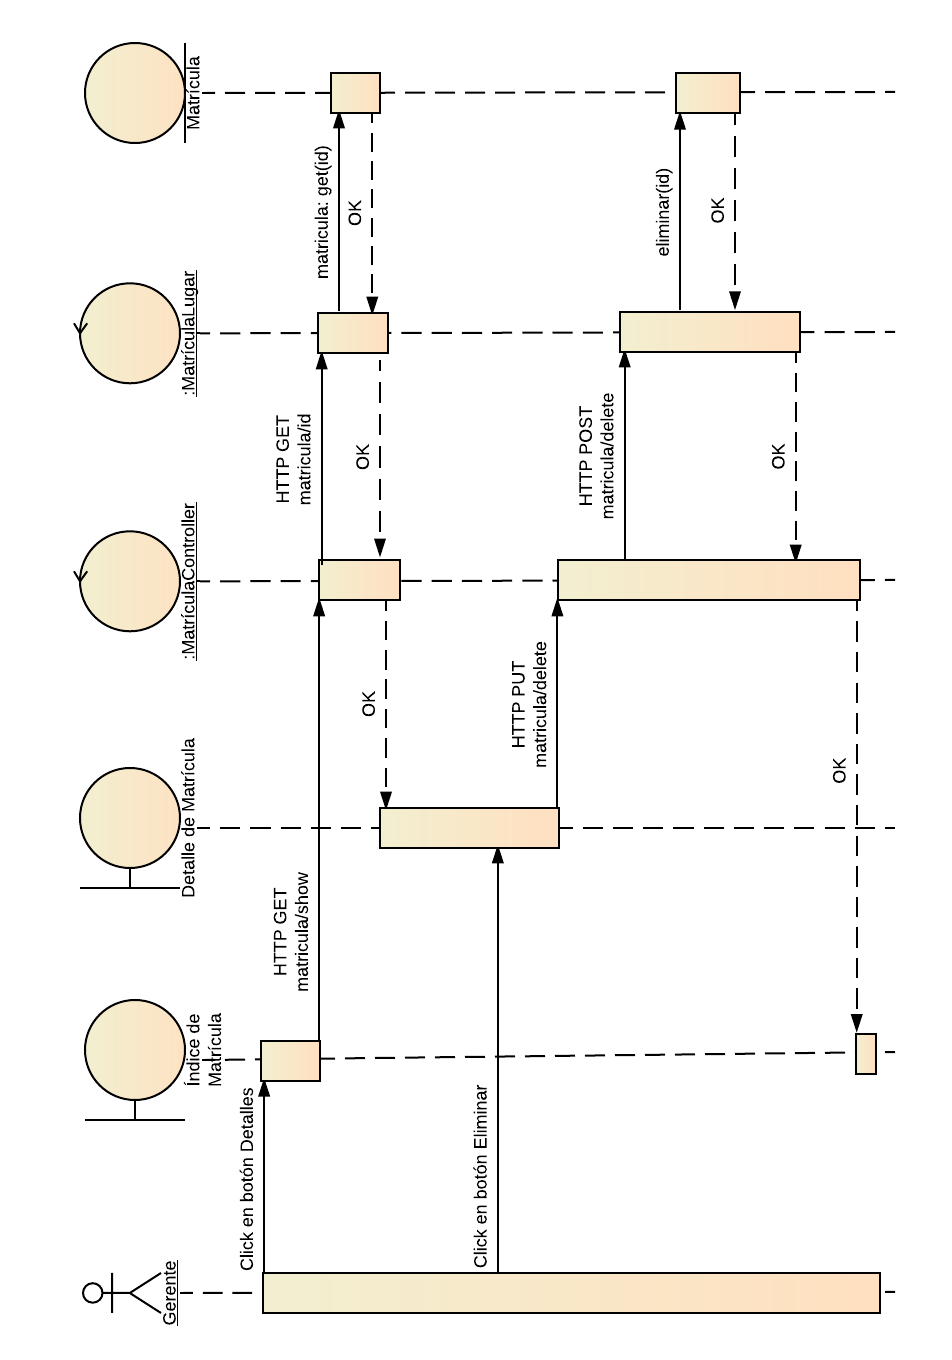
\includegraphics[width=1.2\textwidth]{chapter10/seq-matri-el}
        \caption{Diagrama de Secuencia - Gestionar MatrículaD(3) }
        \label{fig:seq-matri-el}
    \end{figure}
\end{landscape}
    
\section{Gestionar Propietario}

\begin{table}[H]
    \begin{tabular}{@{} p{3cm} p{10cm} @{}} \toprule
    \textbf{Caso de Uso}    & Gestionar Propietario \\ \midrule
    Actor                   & Gerente \\ \cmidrule{1-2}
    Descripción             & El gerente gestiona un Propietario. La información de los propietarios la proporciona otra base de datos. No se permite hacer Altas, Bajas o Modificaciones de esta entidad, solo Lecturas. \\ \cmidrule{1-2}
    Propósito               & El gerente quiere gestionar un Propietario. \\ \cmidrule{1-2}
    Precondiciones          & El gerente inicia su navegador web. \\ 
                            & Existe el Propietario. \\ \cmidrule{1-2} 
    Postcondiciones         & \\ \cmidrule{1-2} 
                            & 1. El gerente visita la página de Propietarios. \\ 
    Curso Básico            & 2. El gerente hace click en el botón Detalles de un Propietario. \\
                            & 2.1 El sistema recupera los datos del Propietario para mostrar la página de detalles. \\ \cmidrule{1-2}
    Excepciones             & \\ \bottomrule
   \end{tabular}
        \caption{Caso de Uso - Gestionar Propietario}
        \label{tab:tabcu-prop}
\end{table}

    \begin{figure}[H]
        \centering
        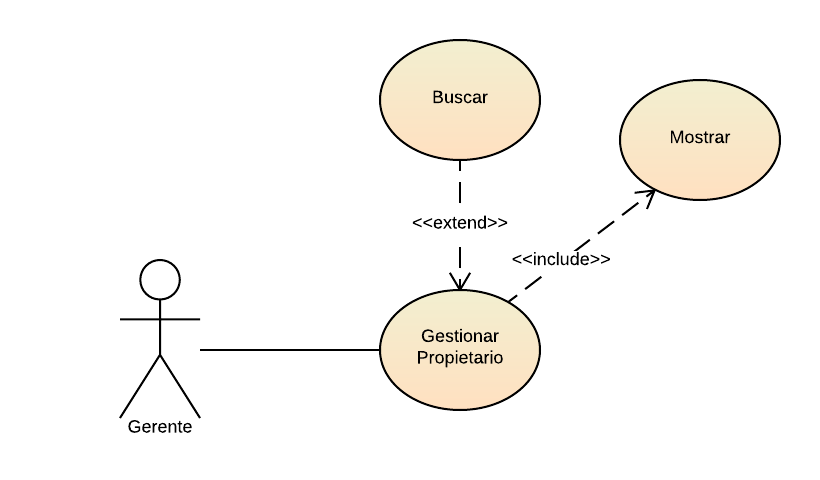
\includegraphics[width=.8\textwidth]{chapter10/uc-prop}
        \caption{Diagrama de Caso de Uso - Gestionar Propietario}
        \label{fig:uc-prop}
    \end{figure}

    \begin{figure}[H]
        \centering
        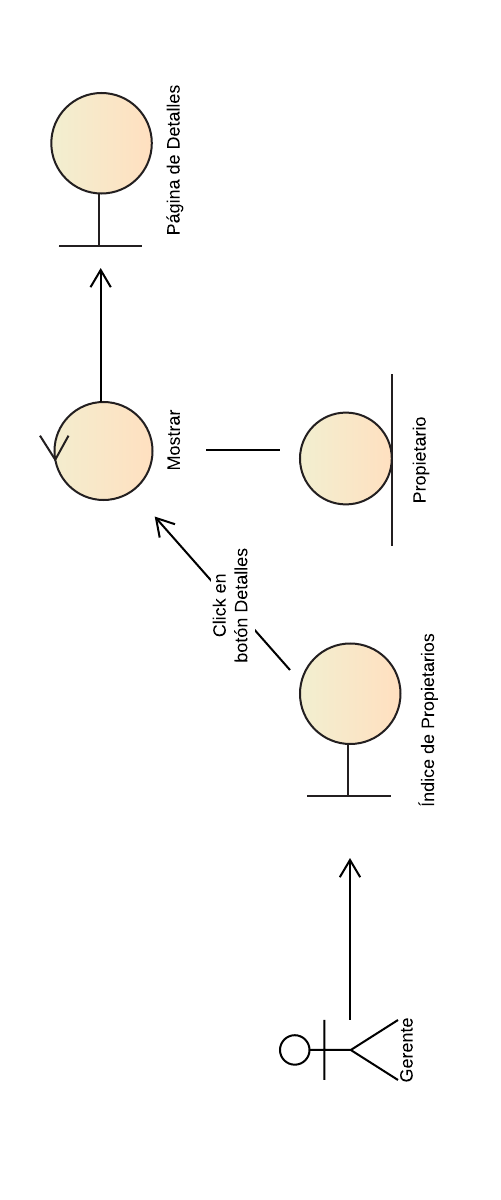
\includegraphics[width=.9\textwidth]{chapter10/rob-prop}
        \caption{Diagrama de Robustez - Gestionar Propietario}
        \label{fig:rob-prop}
    \end{figure}
    \begin{landscape}
        
    \begin{figure}[H]
        \centering
        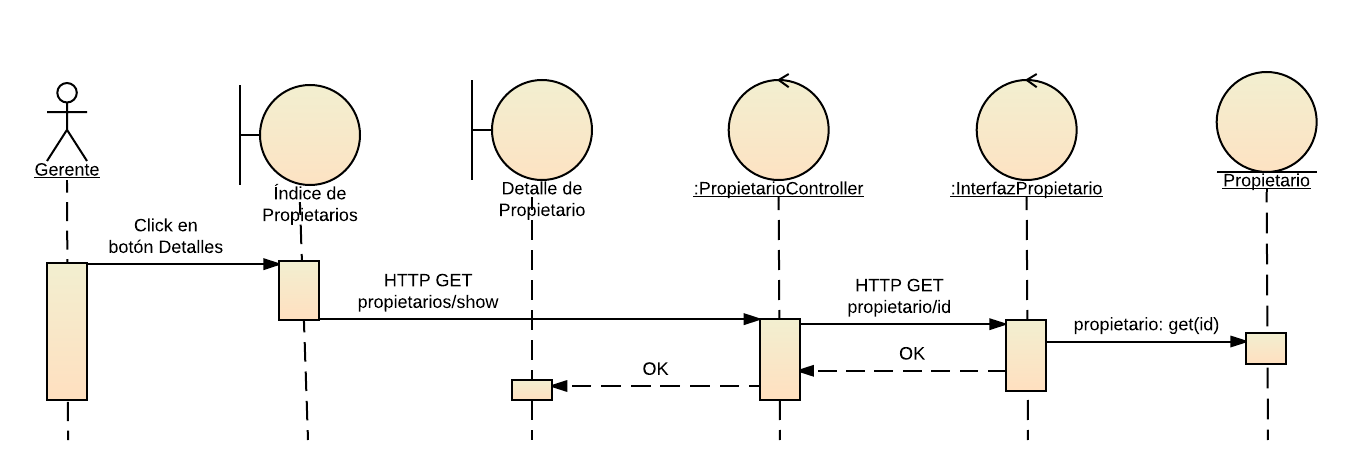
\includegraphics[width=1.2\textwidth]{chapter10/seq-prop}
        \caption{Diagrama de Secuencia - Gestionar Propietario (1) }
        \label{fig:seq-prop}
    \end{figure}
    \end{landscape}
    

\section{Gestionar Conexión a Cámara (Reconocer Matrícula)}

    \begin{longtable}{@{} p{3cm} p{10cm} @{}} \toprule
    \textbf{Caso de Uso}    & Gestionar Conexión a Cámara (Recolectar Vídeo, Reconocer Matrícula) \\ \midrule
    Actor                   & Gerente \\ \cmidrule{1-2}
    Descripción             & El gerente inicia un Servicio Recolector para una cámara registrada. \\ \cmidrule{1-2}
    Propósito               & El gerente quiere que se realicen registros de coincidencias de matriculas a partir del vídeo de las cámaras de seguridad. \\ \cmidrule{1-2}
    Precondiciones          & El gerente inicia su navegador web. \\ 
                            & Existe la cámara. \\ \cmidrule{1-2} 
    Postcondiciones         & Existe un Servicio Recolector para la cámara (la conexión a la cámara esta establecida). \\ \cmidrule{1-2} 
                            & 1. El gerente visita la página de Cámaras. \\ 
                            & 2. El gerente hace click en el botón Conectar. \\
                            & 2.1 El sistema recupera la información de la cámara y la envía a un Servicio Recolector. \\
    Curso Básico            & 2.2. El sistema recolecta el flujo de vídeo y reenvía los cuadros del vídeo a un Servicio de Reconocimiento. \\
                            & 2.3. El Servicio de Reconocimiento procesa los cuadros recibidos y envía  las matriculas reconocidas al Servicio de Coincidencias. \\
                            & 2.4. El Servicio de Coincidencias recupera la información correspondiente a la matricula reconocida y almacena la información asociada. (Caso de Uso: Almacenar Coincidencia) \\ \cmidrule{1-2}
    Excepciones             & \\ \bottomrule
   \caption{Caso de Uso - Gestionar Conexión a Cámara (Reconocer Matrícula)} \label{tab:tabcu-rec}  \\
   \end{longtable}
       
    
    \begin{longtable}{@{} p{3cm} p{10cm} @{}} \toprule
    \textbf{Caso de Uso}    & Gestionar Conexión a Cámara (Almacenar Coincidencia) \\ \midrule
    Actor                   & Gerente \\ \cmidrule{1-2}
    Descripción             & El Servicio de Reconocimiento envía las matriculas reconocidas al Servicio de Coincidencias para ser almacenadas. \\ \cmidrule{1-2}
    Propósito               & Almacenar una coincidencia. \\ \cmidrule{1-2}
    Precondiciones          & Existe el Servicio de Reconocimiento. \\
                            & Existe el Servicio de Coincidencias. \\ \cmidrule{1-2} 
    Postcondiciones         & Se almacenó una nueva coincidencia. \\ \cmidrule{1-2} 
                            & 1. El Servicio de Reconocimiento envía una matricula reconocida al Servicio de Coincidencias. \\ 
    Curso Básico            & 2. El Servicio de Coincidencias busca un propietario asociado a la matricula recibida. \\
                            & 3. El Servicio de Coincidencias busca el lugar asociado a la IP de la cámara recibida. \\
                            & 4. El Servicio de Coincidencias almacena la coincidencia con todos los datos obtenidos, sin referencias a los datos originales, de manera que actúa como un histórico; caso de que los datos de las entidades cambien en el futuro, el registro de la coincidencia no cambiara. \\ \cmidrule{1-2}
    Alternativas            & Caso de que la matricula recibida este incompleta, dado que no concuerda al compararla con una plantilla predeterminada, se marca como irregular. \\ \cmidrule{1-2}
    Excepciones             & Caso de que haya una falla en la base de datos, el sistema no puede registrar la Coincidencia. \\ \bottomrule
   \caption{Caso de Uso - Gestionar Coincidencia} \label{tab:tabcu-rec2}  \\
   \end{longtable}
    
    \begin{figure}[H]
        \centering
        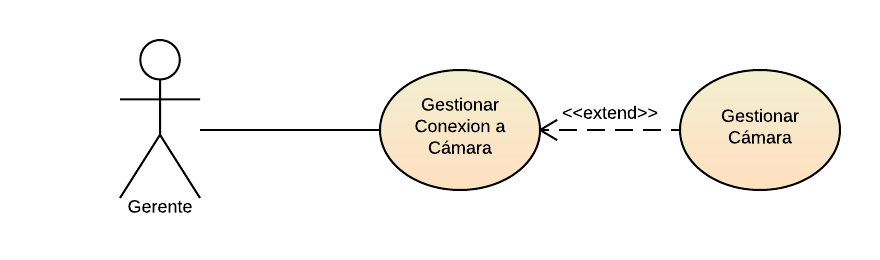
\includegraphics[width=.8\textwidth]{chapter10/uc-rec2}
        \caption{Diagrama de Caso de Uso - Gestionar Conexión a Cámara}
        \label{fig:uc-rec}
    \end{figure}
    \begin{landscape}
        
    \begin{figure}[H]
        \centering
        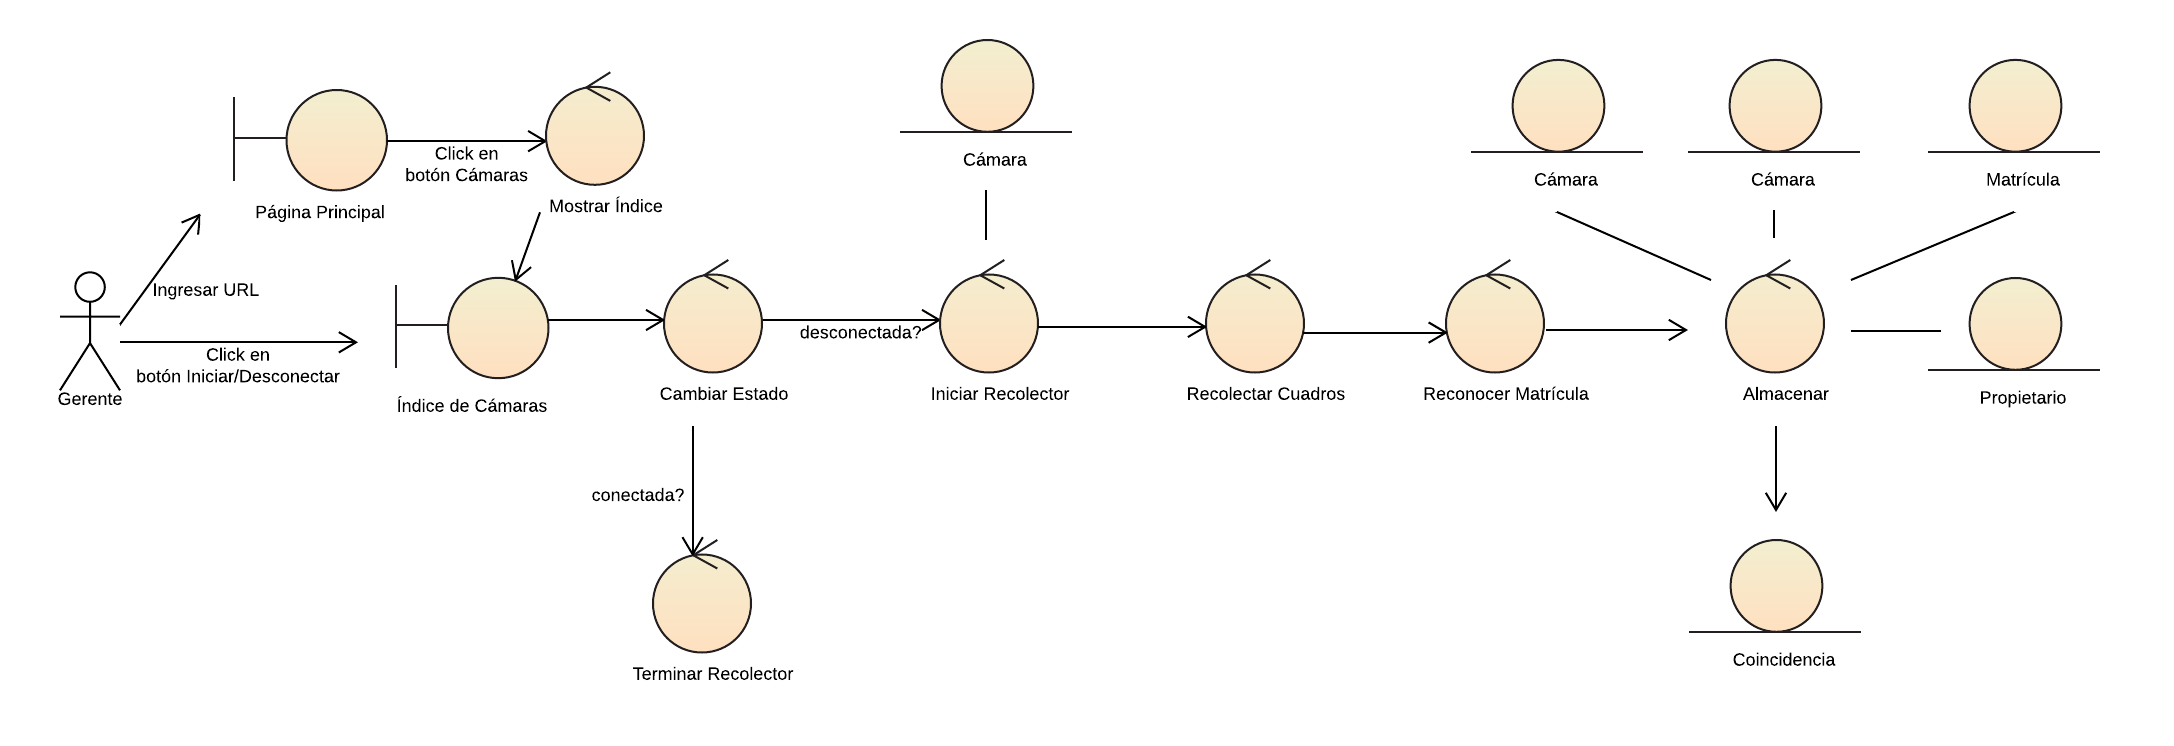
\includegraphics[width=1.4\textwidth]{chapter10/rob-rec}
        \caption{ Diagrama de Robustez - Gestionar Conexión a Cámara}
        \label{fig:rob-rec}
    \end{figure}
    
 \begin{figure}[H]
        \centering
        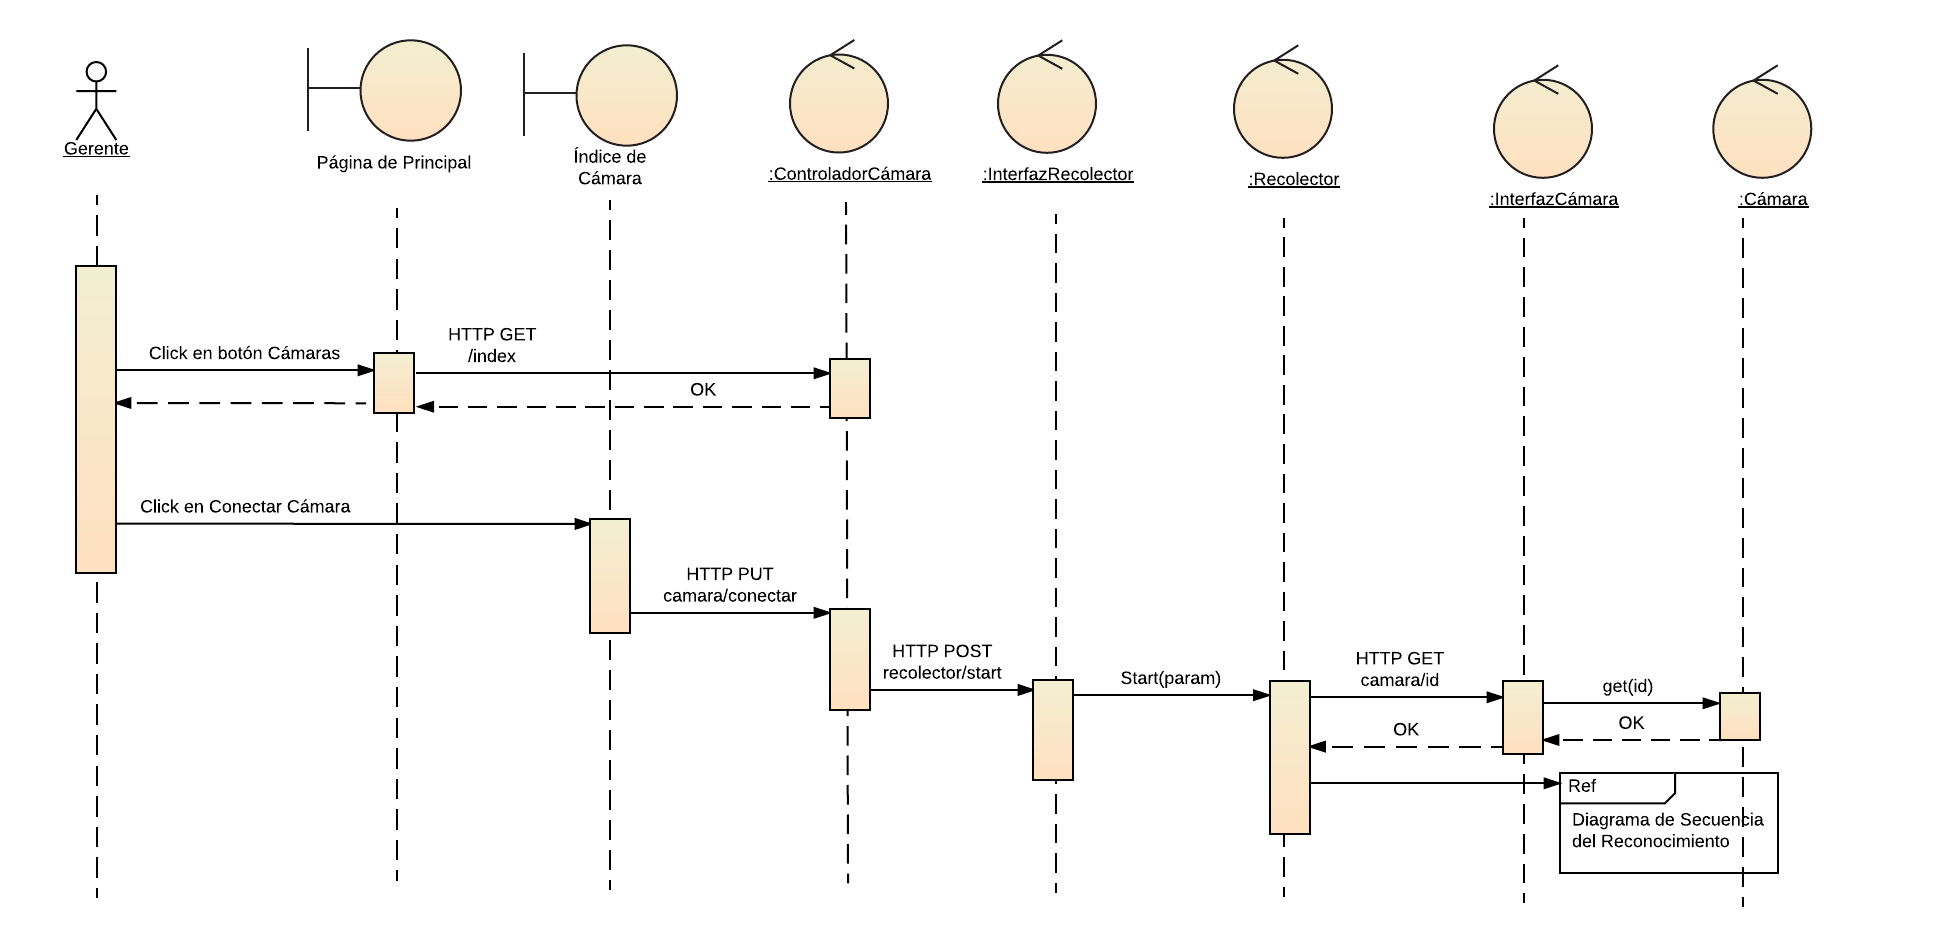
\includegraphics[width=1.3\textwidth]{chapter10/seq-recol}
        \caption{Diagrama de Secuencia - Gestionar Conexión a Cámara (1: Recolección)}
        \label{fig:seq-recol}
    \end{figure}
    
    \begin{figure}[H]
        \centering
        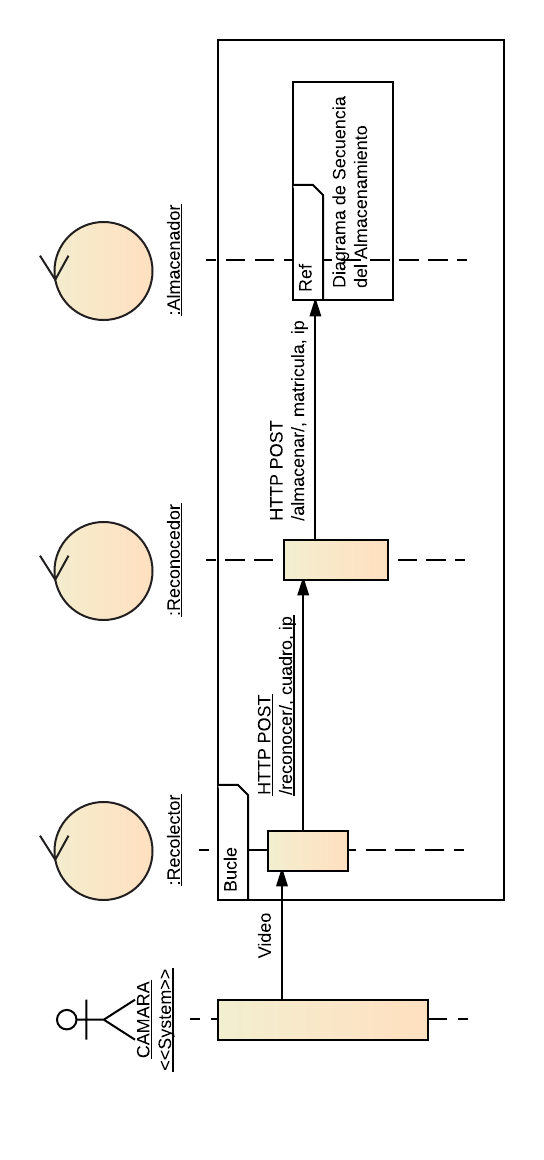
\includegraphics[width=1\textwidth]{chapter10/seq-rec}
        \caption{Diagrama de Secuencia - Gestionar Conexión a Cámara (2: Reconocimiento)  }
        \label{fig:seq-rec}
    \end{figure}
    
    \begin{figure}[H]
        \centering
        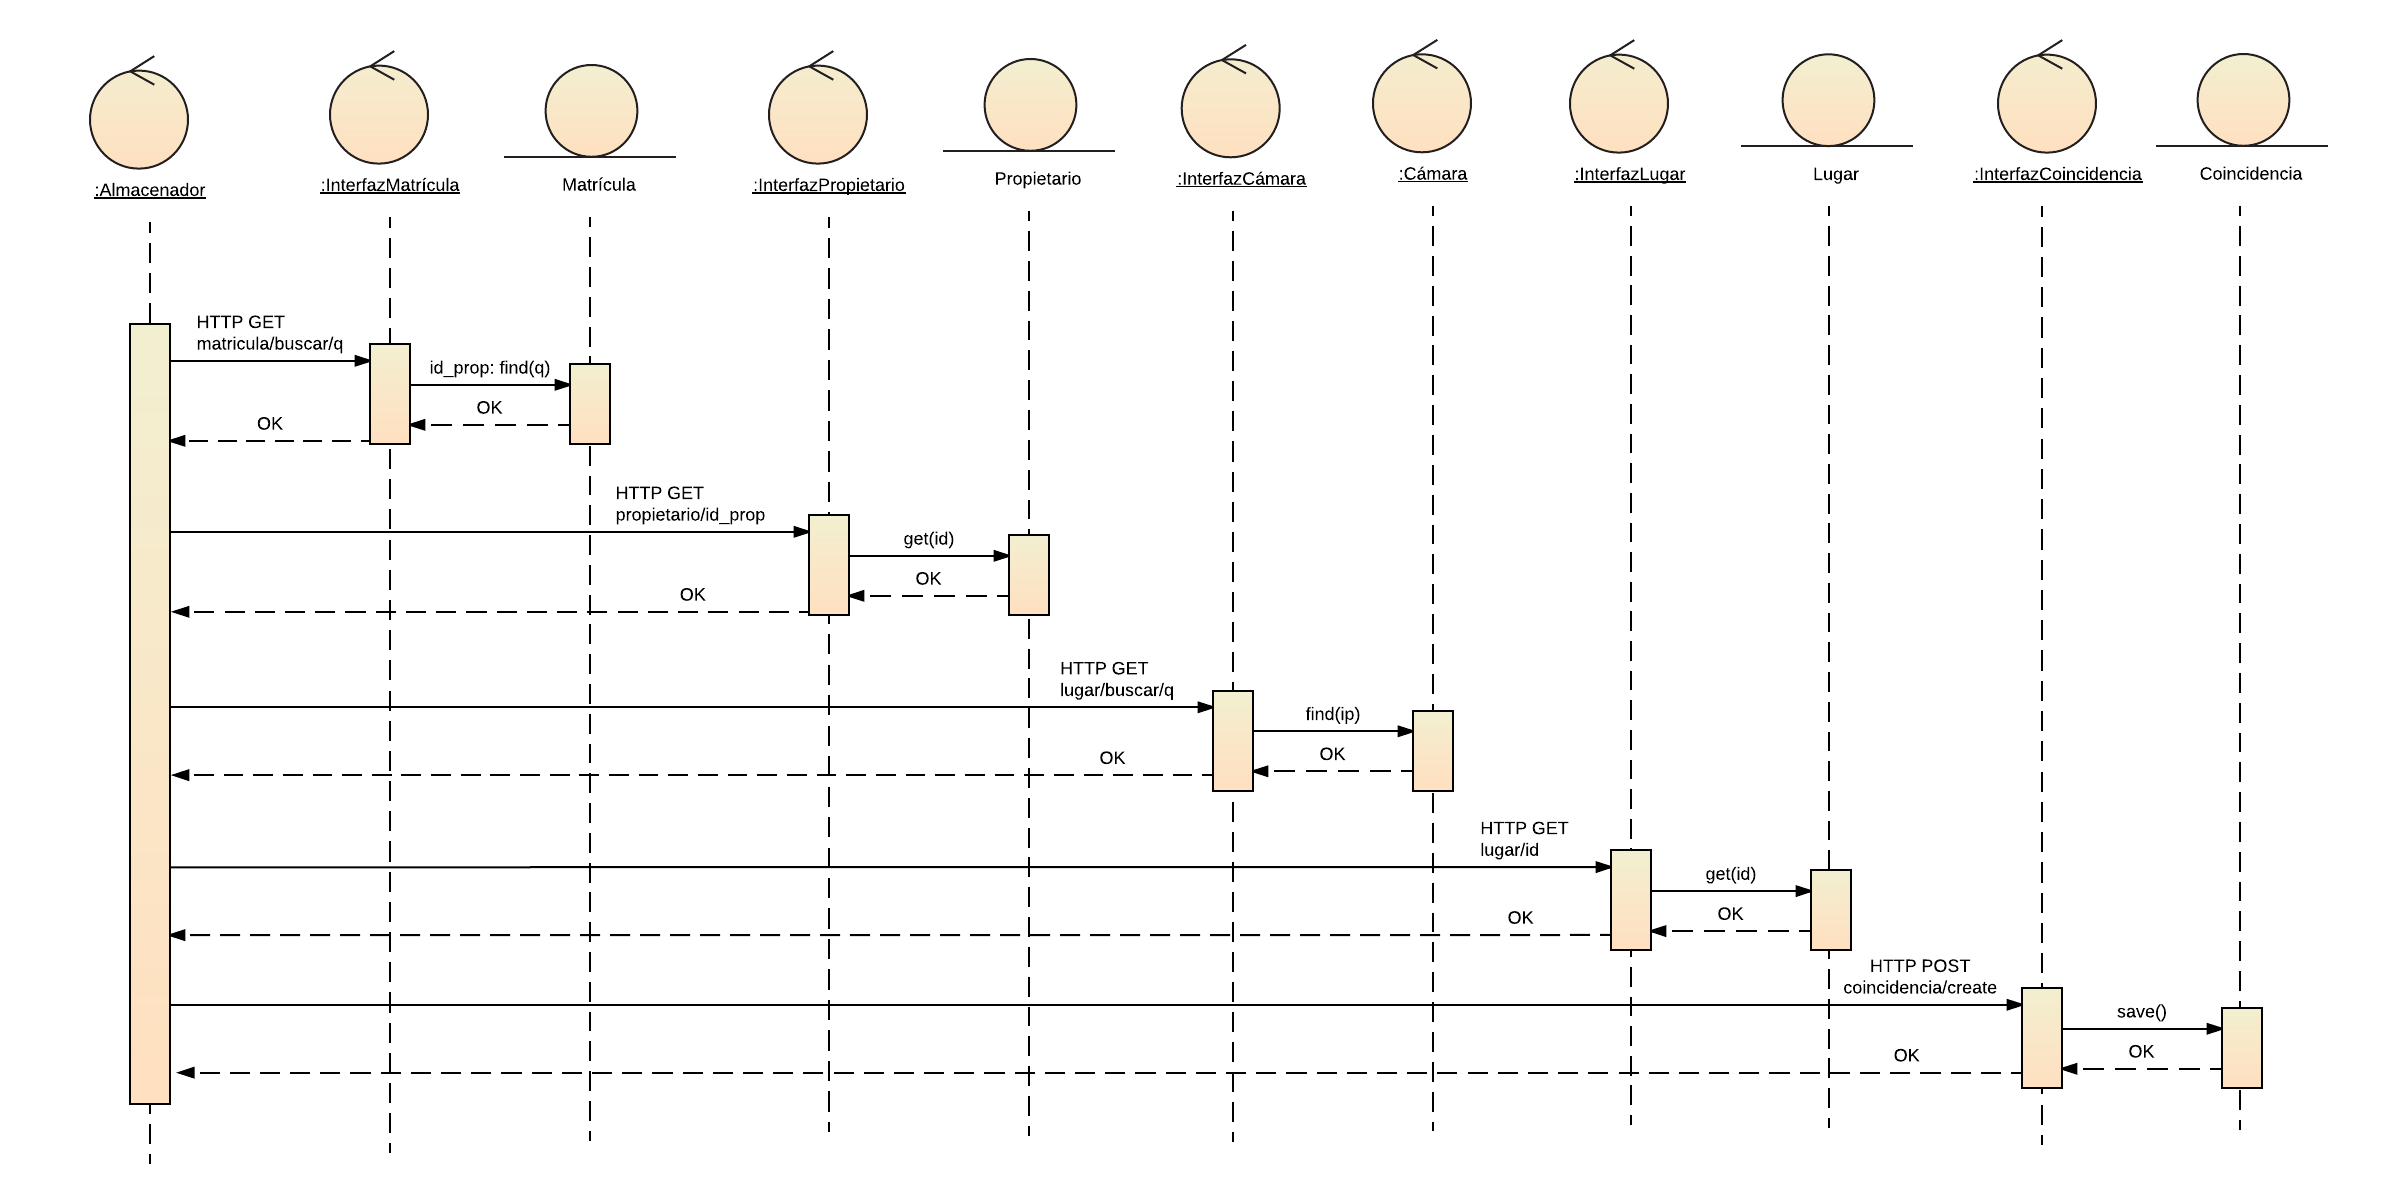
\includegraphics[width=1.3\textwidth]{chapter10/seq-alma}
        \caption{Diagrama de Secuencia - Gestionar Conexión a Cámara (3: Almacenamiento)  }
        \label{fig:seq-alma}
    \end{figure}
    \end{landscape}    
    
\section{Gestionar Coincidencia}

    \begin{longtable}{@{} p{3cm} p{10cm} @{}} \toprule
    \textbf{Caso de Uso}    & Reconocer Coincidencia \\ \midrule
    Actor                   & Gerente \\ \cmidrule{1-2}
    Descripción             & El gerente consulta la información correspondiente a una coincidencia (también llamada registro de matricula, registro de reconocimiento, o resultado de un reconocimiento), y la cual puede corresponder a un propietario que el sistema pueda encontrar o no. \\ \cmidrule{1-2}
    Propósito               & El gerente quiere consultar la información asociada a una coincidencia, esto puede ser imagen, propietario, fecha, lugar, o cámara. \\ \cmidrule{1-2}
    Precondiciones          & El gerente inicia su navegador web. \\ 
                            & Existe la coincidencia. \\ \cmidrule{1-2} 
    Postcondiciones         &  \\ \cmidrule{1-2} 
                            & 1. El gerente visita la página de Coincidencias. \\ 
    Curso Básico            & 2. El gerente hace click en el botón Detalles de una Coincidencia. \\
                            & 2.1 El sistema recupera la información de la coincidencia y muestra la página de Detalles. \\ \cmidrule{1-2}
    Excepciones             & \\ \bottomrule
   \caption{Caso de Uso - Gestionar Coincidencia} \label{tab:tabcu-coin}  \\
   \end{longtable}
    
    \begin{figure}[H]
        \centering
        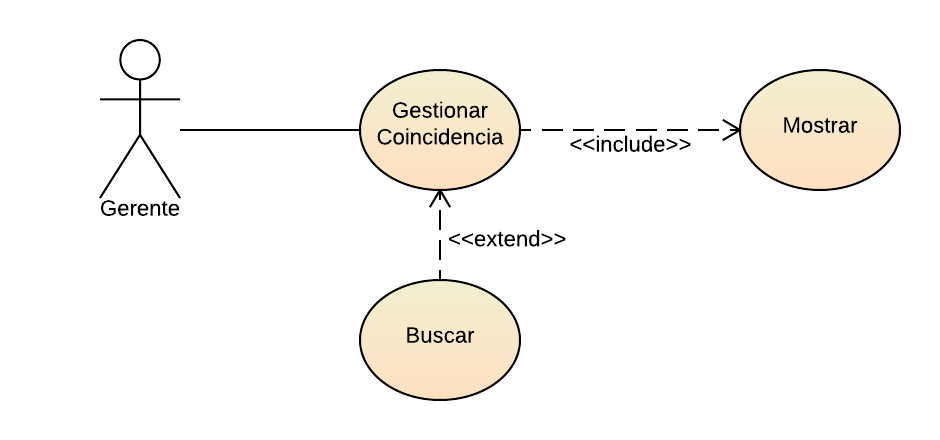
\includegraphics[width=0.7\textwidth]{chapter10/uc-coin}
        \caption{Diagrama de Caso de Uso - Gestionar Coincidencia}
        \label{fig:uc-coin}
    \end{figure}
    
  \begin{figure}[H]
        \centering
        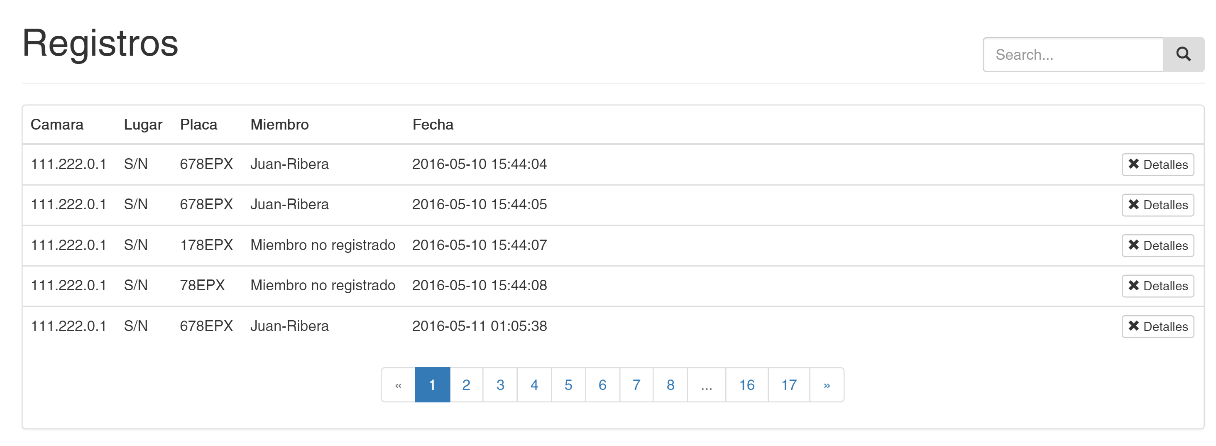
\includegraphics[width=0.85\textwidth]{chapter10/int-coin}
        \caption{Interfaz de Usuario Tentativa - Gestionar Coincidencia}
        \label{fig:int-coin}
    \end{figure}
    
    \begin{figure}[H]
        \centering
        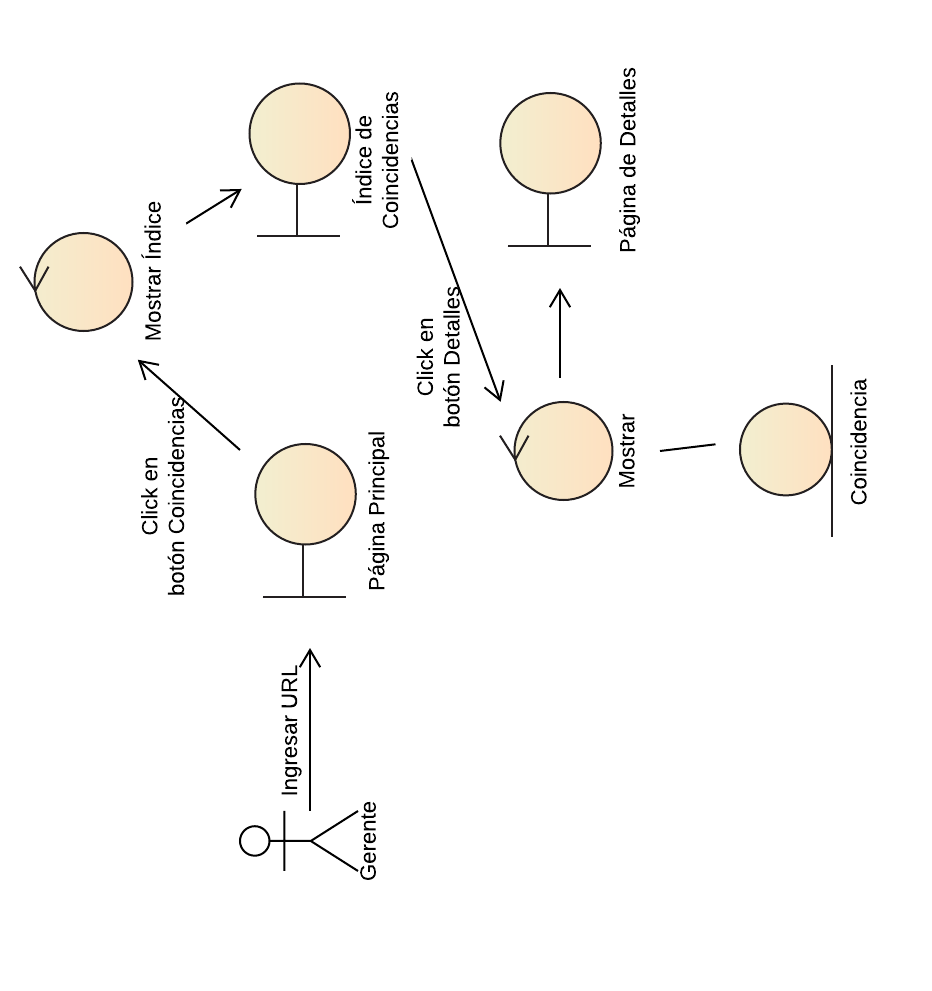
\includegraphics[width=.7\textwidth]{chapter10/rob-coin}
        \caption{Diagrama de Robustez - Gestionar Coincidencia}
        \label{fig:rob-coin}
    \end{figure}
    \begin{landscape}
    
    \begin{figure}[H]
        \centering
        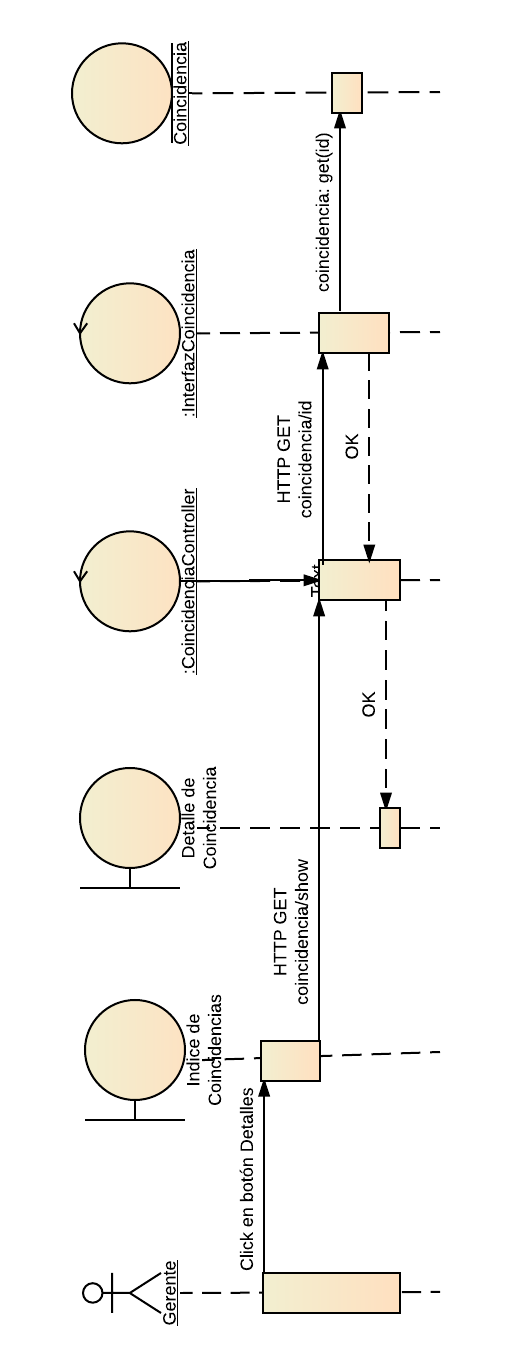
\includegraphics[width=1.2\textwidth]{chapter10/seq-coin}
        \caption{Diagrama de Secuencia - Gestionar Coincidencia }
        \label{fig:seq-coin}
    \end{figure}
    \end{landscape}
    
    
\section{Buscar}
\begin{longtable}{@{} p{3cm} p{10cm} @{}} \toprule
    \textbf{Caso de Uso}    & Buscar\\ \midrule
    Actor                   & Gerente \\ \cmidrule{1-2}
    Descripción             & El gerente consulta información de una entidad de acuerdo a un criterio. \\ \cmidrule{1-2}
    Propósito               & El gerente quiere consultar la información de una coincidencia, propietario, fecha, lugar, o cámara en base a un criterio. \\ \cmidrule{1-2}
    Precondiciones          & El gerente inicia su navegador web. \\ \cmidrule{1-2} 
    Postcondiciones         & El gerente obtuvo una respuesta a su consulta. \\ \cmidrule{1-2} 
                            & 1. El gerente visita la página de la entidad sobre la que quiere buscar (Lugar, Camara, Matricula, Propietario, Coincidencia). \\ 
    Curso Básico            & 2. El gerente ingresa su criterio de búsqueda. \\
                            & 3. El gerente hace click en el botón Buscar. \\
                            & 4. El sistema valida el criterio de búsqueda. \\
                            & 5. El sistema obtiene los resultados en base al criterio. \\
                            & 6. El sistema devuelve los resultados obtenidos. \\ \cmidrule{1-2}
    Alternativas            & El gerente refina su criterio de búsqueda luego de obtener resultados. \\ \bottomrule
    Excepciones             & Dada una falla en la base de datos, el sistema no puede consultar información. \\ 
                            & Dado un criterio invalido, se notifica al gerente los errores que existen\\  \bottomrule
   \caption{Caso de Uso - Buscar} \label{tab:tabcu-coin}  \\
   \end{longtable}
   
\begin{figure}[H]
        \centering
        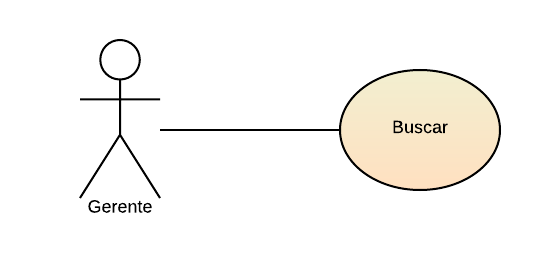
\includegraphics[width=.8\textwidth]{chapter10/uc-buscar}
        \caption{Diagrama de Caso de Uso - Buscar}
        \label{fig:uc-buscar}
    \end{figure}
    
      \begin{figure}[H]
        \centering
        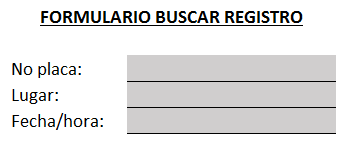
\includegraphics[width=0.85\textwidth]{chapter10/int-buscar-registro}
        \caption{Interfaz de Usuario Tentativa - Gestionar Buscar}
        \label{fig:int-buscar-registro}
    \end{figure}
    
     \begin{figure}[H]
        \centering
        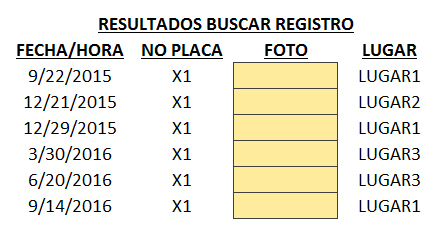
\includegraphics[width=0.85\textwidth]{chapter10/int-buscar-registro-resultados}
        \caption{Interfaz de Usuario Tentativa - Gestionar Buscar}
        \label{fig:int-buscar-registro-resultados}
    \end{figure}
    
 \begin{landscape}
    \begin{figure}[H]
        \centering
        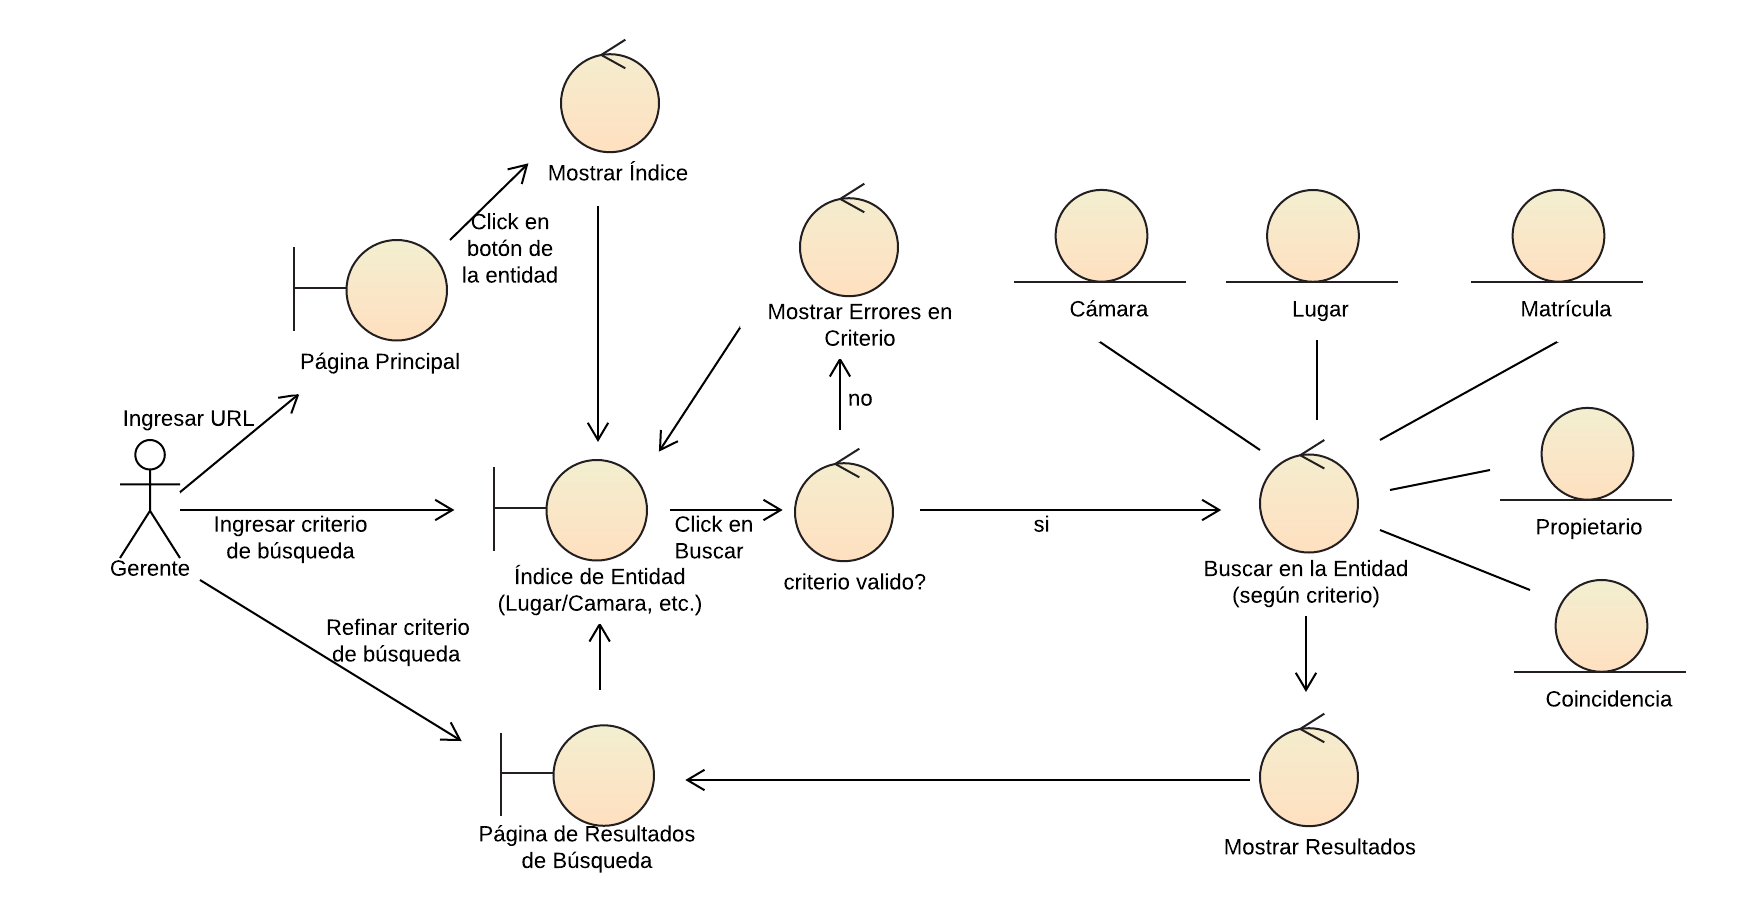
\includegraphics[width=1.2\textwidth]{chapter10/rob-buscar}
        \caption{Diagrama de Robustez - Buscar}
        \label{fig:rob-buscar}
    \end{figure}
    
    \begin{figure}[H]
        \centering
        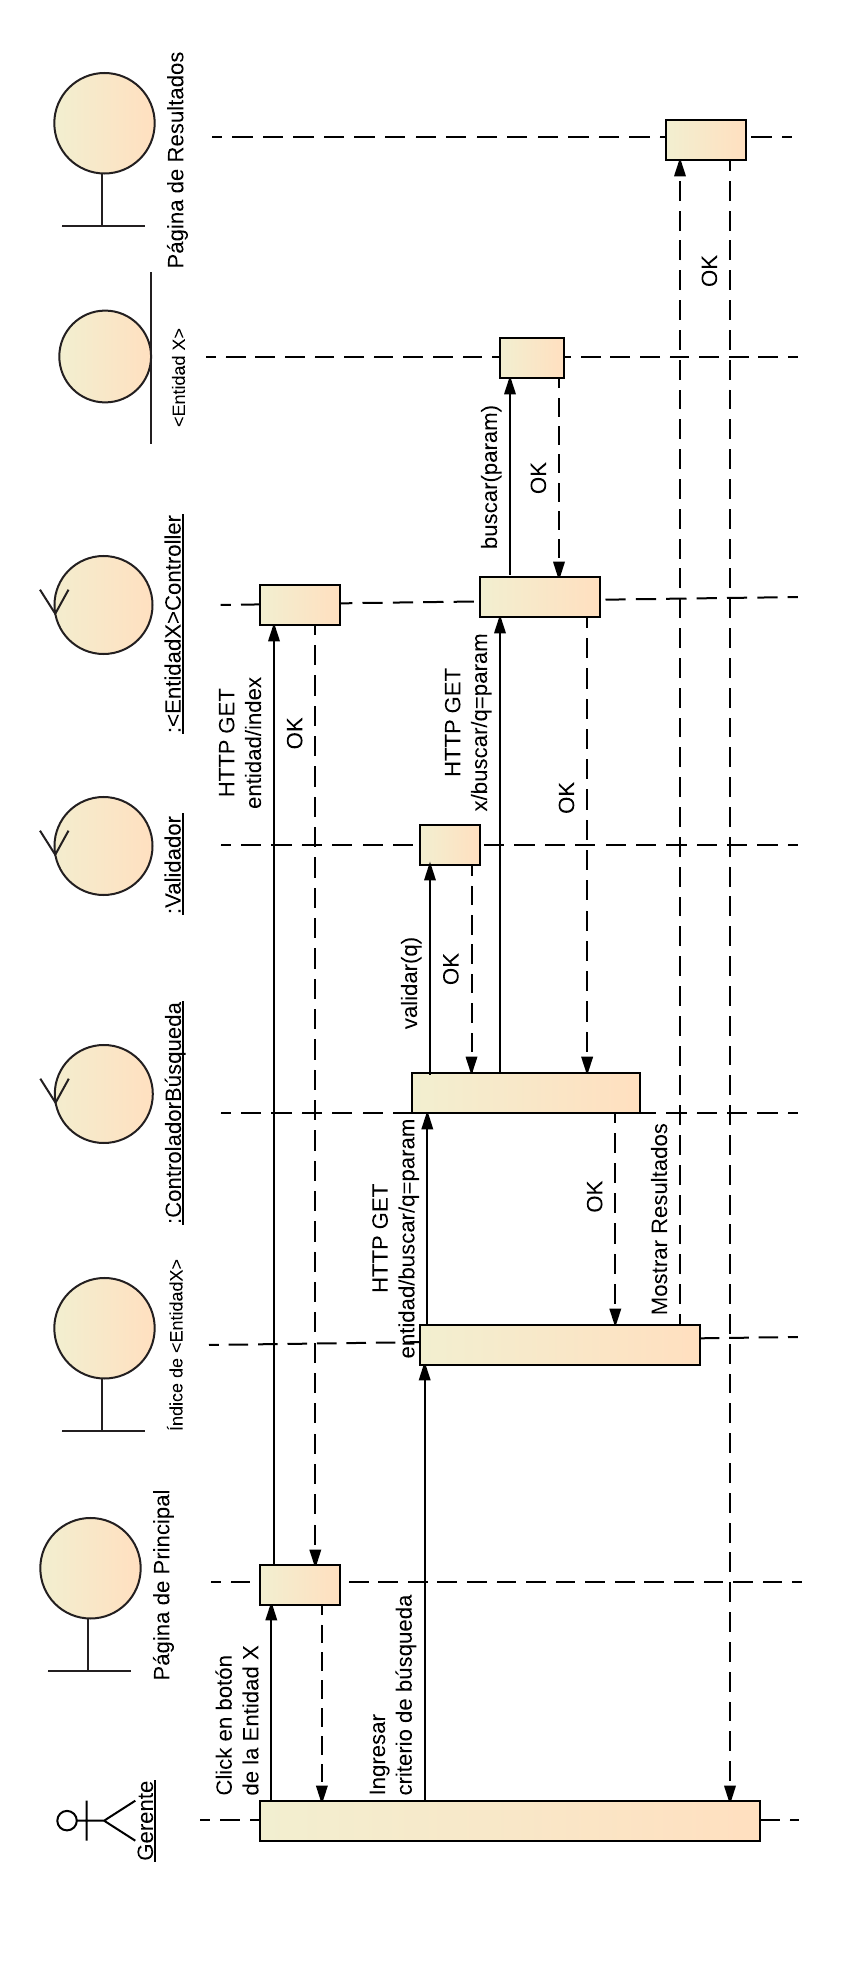
\includegraphics[width=1.3\textwidth]{chapter10/seq-buscar}
        \caption{Diagrama de Secuencia - Buscar }
        \label{fig:seq-buscar}
    \end{figure}
    \end{landscape}
    
\section{Generar Reporte}
\begin{longtable}{@{} p{3cm} p{10cm} @{}} \toprule
    \textbf{Caso de Uso}    & Generar Reporte \\ \midrule
    Actor                   & Gerente \\ \cmidrule{1-2}
    Descripción             & El gerente genera un reporte.\\ \cmidrule{1-2}
    Propósito               & El gerente quiere consultar informacion relevate a traves de un reporte. \\ \cmidrule{1-2}
    Precondiciones          & El gerente inicia su navegador web. Existen resultados a una consulta. \\ \cmidrule{1-2} 
    Postcondiciones         & Se generó un reporte. \\ \cmidrule{1-2} 
                            & 1. El gerente visita la página de Principal \\ 
    Curso Básico            & 2. El gerente hace click en el boton Reportes. \\
                            & 2.1 El sistema muestra la pagina de Reportes. \\
                            & 3. El gerente hace click en el reporte que desea generar. \\
                            & 4. El sistema obtiene los resultados en base al reporte seleccionado. \\
                            & 5. El sistema devuelve el reporte generado. \\ \cmidrule{1-2}
    Excepciones             & El sistema falla en consultar los datos necesarios para el reporte en caso de una falla en la conexion con la base de datos.\\ \bottomrule
   \caption{Caso de Uso - Generar Reporte} \label{tab:tabcu-coin}  \\
   \end{longtable}

\begin{figure}[H]
        \centering
        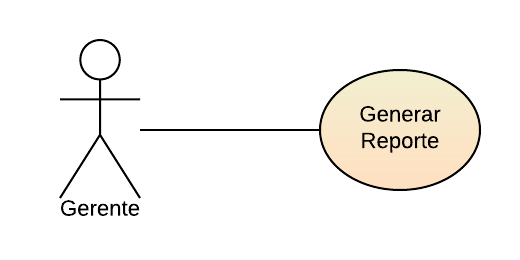
\includegraphics[width=0.5\textwidth]{chapter10/uc-reporte}
        \caption{Diagrama de Caso de Uso - Generar Reporte}
        \label{fig:uc-reporte}
    \end{figure}
          \begin{figure}[H]
        \centering
        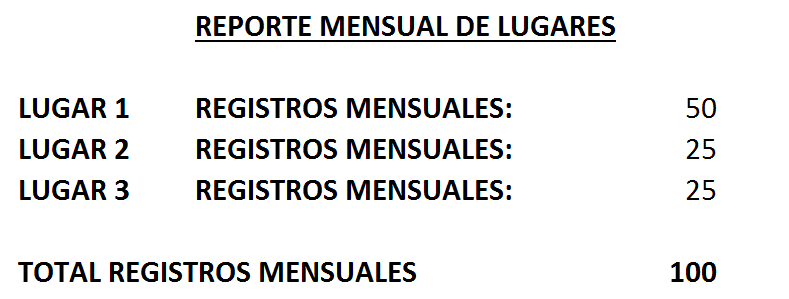
\includegraphics[width=0.85\textwidth]{chapter10/int-reporte-mensual-placas}
        \caption{Interfaz de Usuario Tentativa - Gestionar Reporte (1)}
        \label{fig:int-reporte-mensual-placas}
    \end{figure}
           \begin{figure}[H]
        \centering
        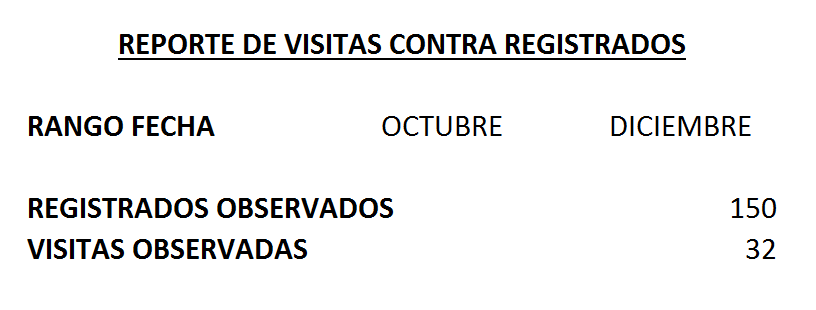
\includegraphics[width=0.85\textwidth]{chapter10/int-reporte-visitantes}
        \caption{Interfaz de Usuario Tentativa - Gestionar Reporte (2)}
        \label{fig:int-reporte-visitantes}
    \end{figure}
    \begin{figure}[H]
        \centering
        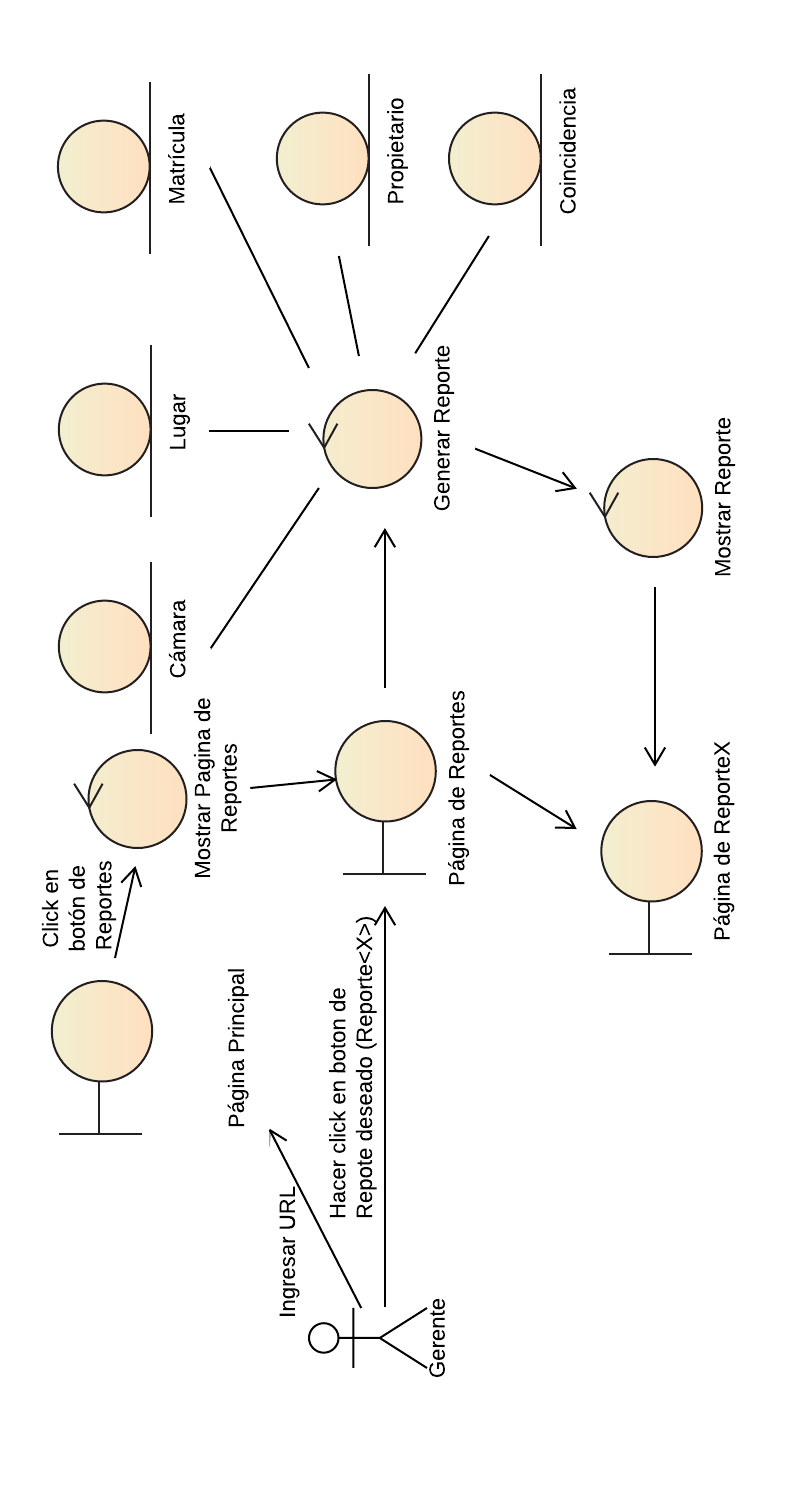
\includegraphics[width=1\textwidth]{chapter10/rob-reporte}
        \caption{Diagrama de Robustez - Generar Reporte}
        \label{fig:rob-reporte}
    \end{figure}
     \begin{landscape}

    \begin{figure}[H]
        \centering
        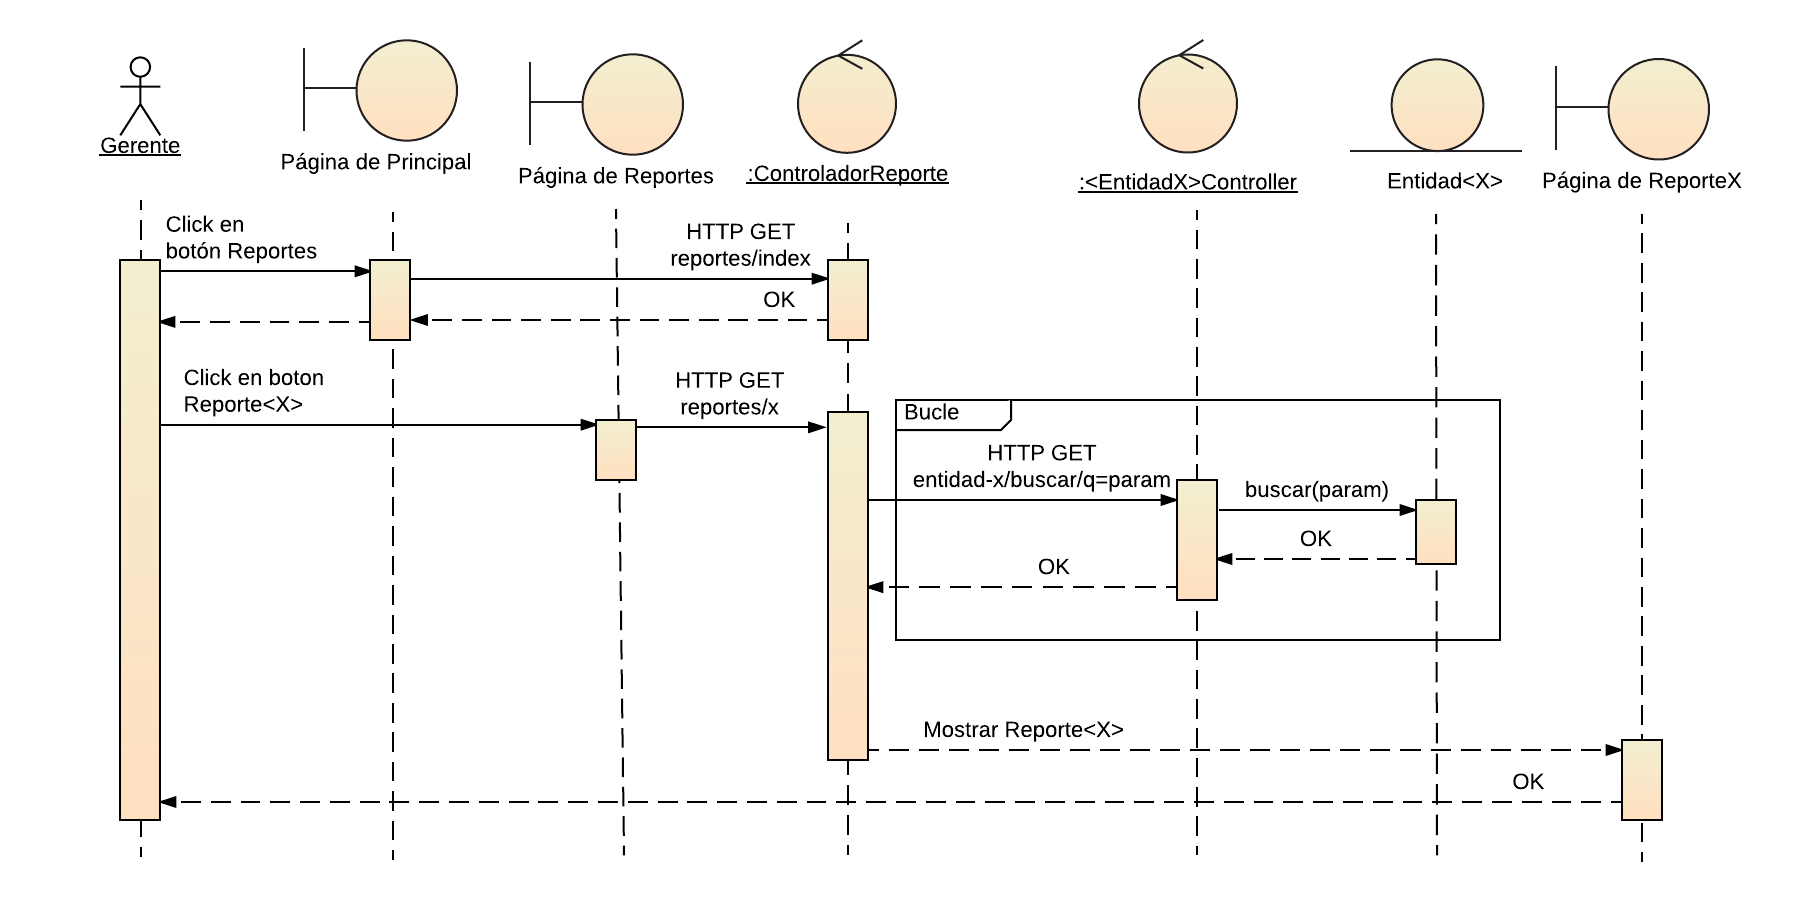
\includegraphics[width=1.3\textwidth]{chapter10/seq-reporte}
        \caption{Diagrama de Secuencia - Generar Reporte }
        \label{fig:seq-reporte}
    \end{figure}
    \end{landscape}
    
\addtocontents{toc}{\protect\setlength{\cftsecnumwidth}{10mm}}